%% Version 4.3.2, 25 August 2014
%
%%%%%%%%%%%%%%%%%%%%%%%%%%%%%%%%%%%%%%%%%%%%%%%%%%%%%%%%%%%%%%%%%%%%%%
% Template.tex --  LaTeX-based template for submissions to the 
% American Meteorological Society
%
% Template developed by Amy Hendrickson, 2013, TeXnology Inc., 
% amyh@texnology.com, http://www.texnology.com
% following earlier work by Brian Papa, American Meteorological Society
%
% Email questions to latex@ametsoc.org.
%
%%%%%%%%%%%%%%%%%%%%%%%%%%%%%%%%%%%%%%%%%%%%%%%%%%%%%%%%%%%%%%%%%%%%%
% PREAMBLE
%%%%%%%%%%%%%%%%%%%%%%%%%%%%%%%%%%%%%%%%%%%%%%%%%%%%%%%%%%%%%%%%%%%%%

%% Start with one of the following:
% DOUBLE-SPACED VERSION FOR SUBMISSION TO THE AMS
\documentclass{ametsoc}

% TWO-COLUMN JOURNAL PAGE LAYOUT---FOR AUTHOR USE ONLY
% \documentclass[twocol]{ametsoc}

%%%%%%%%%%%%%%%%%%%%%%%%%%%%%%%%
%%% To be entered only if twocol option is used

\journal{mwr}

%  Please choose a journal abbreviation to use above from the following list:
% 
%   jamc     (Journal of Applied Meteorology and Climatology)
%   jtech     (Journal of Atmospheric and Oceanic Technology)
%   jhm      (Journal of Hydrometeorology)
%   jpo     (Journal of Physical Oceanography)
%   jas      (Journal of Atmospheric Sciences)	
%   jcli      (Journal of Climate)
%   mwr      (Monthly Weather Review)
%   wcas      (Weather, Climate, and Society)
%   waf       (Weather and Forecasting)
%   bams (Bulletin of the American Meteorological Society)
%   ei    (Earth Interactions)

%%%%%%%%%%%%%%%%%%%%%%%%%%%%%%%%
%Citations should be of the form ``author year''  not ``author, year''
\bibpunct{(}{)}{;}{a}{}{,}

%%%%%%%%%%%%%%%%%%%%%%%%%%%%%%%%

%%% To be entered by author:
% These are not included in ametsoc style file:
\usepackage{amsthm} 
\usepackage{thmtools,thm-restate}
% Useful macros
\newenvironment{mat3}{\left[ \begin{array}{ccc}}{\end{array}\right]}
\newenvironment{mat}{\left[ \begin{array}{ccccccccccccc}}{\end{array}\right]}
\newcommand{\al}[1]{\begin{align}#1\end{align}}
\newcommand{\spl}[1]{\begin{split}#1\end{split}}
\newcommand\nono{\nonumber}
\newcommand\bcm{\begin{mat}}
\newcommand\ecm{\end{mat}}
\newcommand{\haf}{\frac{1}{2}}
\newcommand{\dt}{\Delta t}
\newcommand{\dx}{\Delta x}
\newcommand{\dy}{\Delta y}
\newcommand{\numflux}[1]{\hat{F}\left( \phi_{#1}^{-}, \phi_{#1}^{+}\right)}
\newcommand{\bfv}[1]{\boldsymbol{#1}}
\newcommand{\pbar}[1]{\overline{#1}}
\newtheorem{thm}{Theorem}
\newproof{pf}{Proof}
\newcommand{\beq}{\begin{equation}}
\newcommand{\eeq}[1]{\label{#1}\end{equation}}


%% May use \\ to break lines in title:

\title{Preserving Positivity in Discontinuous Galerkin Methods via Truncation and Mass Aware Rescaling (TMAR)}

%%% Enter authors' names, as you see in this example:
%%% Use \correspondingauthor{} and \thanks{Current Affiliation:...}
%%% immediately following the appropriate author.
%%%
%%% Note that the \correspondingauthor{} command is NECESSARY.
%%% The \thanks{} commands are OPTIONAL.

    %\authors{Author One\correspondingauthor{Author One, 
    % American Meteorological Society, 
    % 45 Beacon St., Boston, MA 02108.}
% and Author Two\thanks{Current affiliation: American Meteorological Society, 
    % 45 Beacon St., Boston, MA 02108.}}

\authors{Devin Light\correspondingauthor{Devin Light, Dept. of Applied Mathematics, University of Washington, Seattle, Washington.}
	     and Dale Durran \thanks{Current affiliation: Dept. of Atmospheric Sciences, University of Washington, Seattle, Washington}}

%% Follow this form:
    % \affiliation{American Meteorological Society, 
    % Boston, Massachusetts.}

\affiliation{University of Washington, Seattle, Washington.}

%% Follow this form:
    %\email{latex@ametsoc.org}

\email{lightd@uw.edu}

%% If appropriate, add additional authors, different affiliations:
    %\extraauthor{Extra Author}
    %\extraaffil{Affiliation, City, State/Province, Country}

%\extraauthor{}
%\extraaffil{}

%% May repeat for a additional authors/affiliations:

%\extraauthor{}
%\extraaffil{}

%%%%%%%%%%%%%%%%%%%%%%%%%%%%%%%%%%%%%%%%%%%%%%%%%%%%%%%%%%%%%%%%%%%%%
% ABSTRACT
%
% Enter your abstract here
% Abstracts should not exceed 250 words in length!
%
% For BAMS authors only: If your article requires a Capsule Summary, please place the capsule text at the end of your abstract
% and identify it as the capsule. Example: This is the end of the abstract. (Capsule Summary) This is the capsule summary. 

\abstract{We describe a uniformly accurate positivity preserving limiter for the advection of scalar tracers based on a discontinuous Galerkin (DG) finite element approximation. The positivity of an unknown tracer field is preserved through the application of a conservative limiter which utilizes a truncation and mass aware rescaling (TMAR) of the local approximating polynomial. The TMAR limiter is straightforward to implement and maintains the original high--order accuracy of the underlying DG scheme while adding only a modest computational expense to each time step. We investigate the performance of the proposed method compared to an existing approach on several standard numerical tests, including a two-dimensional time dependent deformation flow. We observe that the proposed approach performs well in our tests and is particularly suited to higher degree polynomial truncations. }

\begin{document}

%% Necessary!
\maketitle


%%%%%%%%%%%%%%%%%%%%%%%%%%%%%%%%%%%%%%%%%%%%%%%%%%%%%%%%%%%%%%%%%%%%%
% MAIN BODY OF PAPER
%%%%%%%%%%%%%%%%%%%%%%%%%%%%%%%%%%%%%%%%%%%%%%%%%%%%%%%%%%%%%%%%%%%%%
%

%% In all cases, if there is only one entry of this type within
%% the higher level heading, use the star form: 
%%
% \section{Section title}
% \subsection*{subsection}
% text...
% \section{Section title}

%vs

% \section{Section title}
% \subsection{subsection one}
% text...
% \subsection{subsection two}
% \section{Section title}

%%%
% \section{First primary heading}

% \subsection{First secondary heading}

% \subsubsection{First tertiary heading}

% \paragraph{First quaternary heading}

\section{Introduction} \label{sec:intro}
Discontinuous Galerkin (DG) finite element methods are an increasingly popular means of producing numerical approximations to systems of hyperbolic conservation laws. Methods from this family are attractive because they are high--order accurate, geometrically flexible, $h$--$p$ adaptive, compactly defined, and scale well on distributed memory systems \citep{Giraldo:2002aa}. In this paper we will consider DG approximations to the one- and two-dimensional transport of an inert scalar tracer $\psi(\bfv{x},t)$ which is advected by a flow with velocity $\bfv{u}(\bfv{x},t)$ through a spatial domain $\Omega$ which has suitable boundary conditions,
\al{ \label{eq:transp}
&\frac{\partial}{\partial t} \psi(\bfv{x},t) + \nabla \cdot \left( \bfv{u}(\bfv{x},t)\, \psi(\bfv{x},t) \right) = 0, \quad (\bfv{x}, t) \in \Omega \times \mathbb{R}^+ \\
&\psi(\bfv{x},t=0) = \psi_0(\bfv{x}). \nono
}

A classic consequence of the advection equation is if the velocity field is non-divergent (i.e. $\nabla \cdot \bfv{u} = 0$) then equation \eqref{eq:transp} is equivalent to the following non-conservative equation
\al{ \label{eq:noncons}
&\frac{\partial}{\partial t} \psi(\bfv{x},t) + \bfv{u}(\bfv{x},t) \cdot \nabla  \, \psi(\bfv{x},t) = 0.
}
Analytic solutions to \eqref{eq:noncons} satisfy a boundedness relationship determined by the initial data $\psi_0(\bfv{x})$. For example, if $m \leq \psi_0 \leq M$ for all $\bfv{x} \in \Omega$ then $\psi(\bfv{x},t)$ will also satisfy $m \leq \psi(\bfv{x},t) \leq M$ for all $t \geq 0$ and all $\bfv{x} \in \Omega$.  However, even in divergent flows in which \eqref{eq:noncons} is not generally equivalent to the original equation \eqref{eq:transp}, the solutions to \eqref{eq:transp} will nevertheless still satisfy a nonnegativity condition $0 \leq \psi(\bfv{x},t)$, assuming that the initial data is also nonnegative. Beyond emulating a physical quality of the analytic solution, maintaining a nonnegative numerical solution can be of great importance to stability, particularly when \eqref{eq:transp} is integrated as part of a more complicated system which can involve nonlinear source terms. In practice, these forcing effects are often updated separately from the advective step via techniques like operator splitting. An example of this type of a problem in a geophysical context is the reactive transport system considered in \citet{Lauritzen:2015aa}, where $\psi$ represents the mixing ratio of a chemical species of chlorine which should ideally remain nonnegative throughout the integration. If spurious negative undershoots are generated in the approximate solution the resulting negative species concentrations can quickly destabilize the method by inducing reactions which would otherwise be impossible \citep{durran2010numerical}. As a result it is vitally important for stability purposes, rather than accuracy, that the numerical solutions to \eqref{eq:transp} maintain the nonnegativity of the initial data where applicable. However, as a consequence of Godunov's theorem, when a high--order method such as a DG scheme is used to simulate the transport of data which contains poorly resolved steep gradients, Gibbs--like oscillations can generate spurious negatives which will then lead to instabilities if left unchecked. Therefore it is necessary to augment the standard DG approach with some limiting techniques for positivity preservation.

Many existing limiting techniques for DG schemes can be adapted to enforce nonnegativity of the solution. Proposed limiters have taken a variety of approaches towards limiting such as adding artificial viscosity \citep{hartmann2002,persson2006}, extending classical TVB limiters \citep{cbShuRKDG-2,cbShuRKDG-3}, WENO DG limiters \citep{qiu-WENODG-1,qiu-WENODG-2,qiu-WENODG-3}, and a posteriori limiting \citep{dumbser2015}. For a brief review of a selection of these methods, see \citet{dumbser2015}. Another widely used method for keeping DG approximations to conservation laws nonnegative is to adapt the bounds preserving limiter proposed in \citet{Zhang2010,Zhang:2011aa}, hereafter the ZS limiter, for use as a positivity preserving limiter (see \citet{Rossmanith:2011aa,Qiu:2011aa,Guo:2013aa}). The ZS limiter modifies the numerical solution for nonnegativity in two stages using a conservative linear rescaling originally proposed in \citet{Liu:1996aa}. When combined with a suitable time step condition, the ZS rescaling guarantees the nonnegativity of the approximate solution. The ZS limiter is attractive for several reasons: it preserves high--order accuracy, is locally defined, and is straightforward to implement alongside existing methods \citep{Zhang2010}. 

We propose an alternative limiter which enjoys many of the same benefits as the ZS limiter but can perform better for higher degree polynomial approximations with similar computational effort. Like the ZS approach, nonnegativity is preserved in two stages. In the first stage a flux-corrected transport (FCT) adjustment is made to the numerical fluxes just before the forward step so that the mean value of the approximation over the element remains nonnegative throughout the update. After the means have been updated, a second modification to the polynomial is made which corrects for any remaining spurious negatives within the element. The primary difference between the two methods is where the ZS limiter uses a linear rescaling to make both adjustments, the proposed method implements a nonlinear adjustment to the polynomial which truncates spurious negatives to zero while simultaneously modifying the remaining nodes to maintain conservation. 

The remainder of the paper is structured as follows. In Section \ref{sec:dg} we oultine some preliminary DG terminology and methodolgy. Section \ref{sec:pp1d} presents the proposed positivity preserving DG scheme for the one-dimensional problem and analyzes its impact on convergence. In Section \ref{sec:pp2d} we describe an extension of this approach to two-dimensional problems. Section \ref{sec:numTest} examines the empirical performance of the proposed limiter on several one-dimensional and two-dimensional test problems. Section \ref{sec:Efficiency} investigates the computational expense of implementing the proposed limiter. Finally, Section \ref{sec:conc} contains our conclusions.

\section{Preliminaries} \label{sec:dg}
\subsection*{Spatial discretization}
The proposed method will be based on the standard Runge-Kutta DG (RKDG) formulation presented in \citet{Hesthaven:2007aa}, \citet{durran2010numerical}, and \citet{Lauritzen:2011aa}. Let $S^h$ be a Cartesian discretization of the computational domain $\Omega$ into $h$ elements with width $\dx$. Define $V_N^h$ as the vector space of piecewise polynomials on $S^h$ which is formally given by $V_N^h = \left\{ p : p\big|_{s_i} \in \mathbb{P}_N(s_i) \, \forall s_i \in S^h \right\}$ where $\mathbb{P}_N(s_i)$ is the space of polynomials in $s_i$ up to degree $N$. Let $\phi(x,t) \in V_N^h$ be the DG approximation to the solution of \eqref{eq:transp}. We express this approximation at time $t^n$ within element $s_i$ as an expansion of basis polynomials $\varphi_k(x)$,
\al{ \label{polyExp}
\phi_{s_i}^n(x)  = \sum \limits_{k} a_{i,k}(t^n) \, \varphi_k (x) \,\,\text{ for }\,\, x\in s_i,
}
where the summation is taken over the total number of basis polynomials. For one-dimensional problems, popular choices for the basis polynomials are either Legendre polynomials or Lagrange interpolating polynomials. Methods utilizing Lagrange polynomials  have further options for the set of points through which the basis polynomials interpolate; for this paper we will use the $N+1$ Gauss-Legendre-Lobatto (GLL) quadrature nodes $x_k$ that have been mapped to $s_i$ and have corresponding quadrature weights $w_k$ where $k=0,...,N$. Discontinuous Galerkin methods which implement a Legendre basis are sometimes known as modal methods (because the coefficients $a_{i,k}$ represent the modes of the Legendre polynomial), while methods using Lagrange polynomials are called nodal methods (because the coefficient $a_{i,k}$ coincides with the value of $\phi_{s_i}^n(x)$ at the node $x_k$). When solving problems in two or higher space dimensions, we will extend the one-dimensional basis functions via tensor products.

The Discontinuous Galerkin approximation to equation \eqref{eq:transp} is obtained by multiplying the differential equation by a test function $\varphi_k(x)$ and formally integrating by parts over $s_i$ to get
\al{ \label{weak2}
\frac{d}{dt} \int_{s_i} \phi_{s_i}^n(x) \varphi_k(x) \,dx = \int_{s_i}  \phi_{s_i}(x,t) \, \bfv{u}(x,t) \cdot \nabla \varphi_k(x) \, dx - \int_{\partial s_i} \phi_{s_i}(s,t) \bfv{u}(s,t) \cdot \bfv{n} \varphi_k(s)ds \quad \forall \varphi_k \in V_N^h
}
%\al{ \label{weak1}
%\frac{d}{dt} \int_{s_i} \phi_{s_i}^n(x) \varphi_k(x) \,dx = - \int_{s_i} \nabla \cdot \left( \bfv{u}(x,t)\, \phi_{s_i}(x,t) \right) \varphi_k(x) \, dx \quad \forall \varphi_k \in V_N^h.
%}
%Formally integrating by parts this becomes

where $\bfv{n}$ is the outward-facing unit normal on the boundary of $s_i$. The boundary term in \eqref{weak2} is not precisely defined because $\phi$ is discontinuous across element interfaces. To remedy this, the exact flux along the boundary is replaced with the numerical flux function $\hat{F}( \cdot, \cdot )$. A simple choice for scalar transport is the upwind flux
\beq 
\numflux{h} 	= \begin{cases} 
					\bfv{u}\phi_{h}^{-} & \mbox{if } \bfv{u}\cdot\bf{n}\ge 0 \\
					\bfv{u}\phi_{h}^{+} & \mbox{if } \bfv{u}\cdot\bf{n} < 0 
				 \end{cases}.
\eeq{numflux}
where $\phi_{h}^{-}$ and $\phi_{h}^{+}$ are the DG approximations to the edge value from within $s_i$ and $s_{i+1}$, respectively. Although upwind fluxes give only a first-order scheme in standard finite volume methods, they do not adversely affect the spectral accuracy of DG schemes. 

Substituting the expansion \eqref{polyExp} into \eqref{weak2} gives the matrix equation
\al{ \label{matrixEqn}
\bfv{M} \, \frac{d\bfv{a}_i}{dt} = \bfv{G}
}
where $\bf{a_i}$ is the vector of expansion coefficients, $\bfv{M}$ is the mass matrix with entries
\al{ \label{massMatrix}
\bfv{M}_{j,k} = \int_{s_i} \varphi_j(x) \varphi_k(x) \, dx,
}
and $\bfv{G}$ is the vector
\al{ \label{gDef}
\bfv{G}_k = \int_{s_i}  \phi_{s_i}(x,t) \, \bfv{u}(x,t) \cdot \nabla \varphi_k(x) \, dx - \int_{\partial s_i} \numflux{s_i} \cdot \bfv{n} \varphi_k(s)ds.
}
The integrals in \eqref{massMatrix} and \eqref{gDef} are approximated using numerical quadrature. Modal methods use a high order accurate Gaussian rule, while nodal approaches opt instead for the natrual GLL rule defined by the interpolation nodes. As a consequence of the orthogonality of Legendre polynomials, $\bfv{M}$ is diagonal for modal methods which simplifies the solution of \eqref{matrixEqn}. On the other hand, if the mass matrix integral in \eqref{massMatrix} for a nodal method were to be evaluated exactly $\bfv{M}$ would not be diagonal and solving \eqref{matrixEqn} would require a matrix inversion at each stage in a time step. However, if the GLL integration rule implied by the underlying interpolation grid (which is not exact) is used to approximate the integrals, the resulting mass matrix will be diagonal. This technique is sometimes known as mass lumping \citep[p. 57]{kgs2013spectral}. To evolve forward in time, the semi-descrete system in \eqref{matrixEqn} is integrated using a strong stability preserving Runge-Kutta (SSPRK) method. For the numerical simulations performed in this paper, the three-stage, third-order SSPRK method from \citet{Gottlieb:2009aa} is used.

When solving a $d$--dimensional problem, an individual element has $(N+1)^d$ spatial degrees of freedom when using a tensor product basis. Throughout this paper, we will define a discrete sub--element data representation which uses the same number of degrees of freedom for the purpose of defining where the numerical solution should be nonnegative. For nodal methods this representation will be the local approximation evaluated at the tensor product GLL nodes. As a consequence of Lagrange interpolation these values coincide exactly with the expansion coefficients themselves. For modal methods we will use an uniform Cartesian subgrid denoted $s_{ik}$, $k=1,\dots,(N+1)^d$ such that $s_i = \cup_{k} s_{ik}$. Then we represent the sub--element solution with the collection of subcell averages $\phi_{ik}$ given by
\al{\label{subcellAvg}
\phi_{ik}^n = \frac{1}{|s_{ik}|} \int_{s_{ik}} \phi_{s_i}^n(\bfv{x}) \, d\bfv{x}, \quad \forall s_{ik} \in s_i.
}
Equation \eqref{subcellAvg} can be also be written in terms of a projection operator $P$ as $\bfv{\phi}_i = P \bfv{a}_i$. After limiting the sub--element solution (when necessary) we must apply a reconstruction operator $R$ to translate the sub--cell modifications back to the polynomial coefficients at the end of the time step. As a result of our sub--element reconstruction using the same number of degrees of freedom as the original polynomial approximation, the matrix representation of $P$ will be nonsingular and $R$ will correspond to its inverse $P^{-1}$. 

\subsection*{ZS Positivity Preservation}
The ZS limiter is a two-stage bounds preserving limiter first proposed for scalar conservation laws in \citet{Zhang2010}.  In the first stage, the local polynomial approximation is modified so that its mean value over a cell is nonnegative after the forward update. Then in the second stage the polynomial is adjusted again so that the final approximation is positive within the element. If $\phi$ is the local DG approximation for the element $s_i$ with average value $\pbar{\phi}$, the modified polynomial $\phi^*$ for either stage will be of the form
\al{ \label{zsRescale}
\phi^* = \theta \left( \phi - \pbar{\phi} \right) + \pbar{\phi}, \quad \theta = \min \left\{ \frac{m_0 - \pbar{\phi}}{m - \pbar{\phi}}, 1 \right\},
}
where 
\al{
m_0 = \min_{x\in s_i} \psi(x), \quad m = \min_{x \in \Gamma_i} \phi(x).
}
The set $\Gamma_i$ is the collection of points over which the minimum value of $\phi(x)$ is taken and may be different between the two stages. For computational efficiency, the first stage $\Gamma_i$ should contain the minimum number of points which will still ensure that the means remain nonnegative. It was shown in \citet{Zhang:2011aa} that for one-dimensional problems $\Gamma_i$ must consist of at least the two edge points of the element and a third point whose value can be written in terms of the values of $\phi$ at the edges. When extended to two dimensional problems with Cartesian elements, $\Gamma_i$ will consist of a collection of points along the edges of the element plus an additional internal point $\bfv{x}^*$ whose value $\phi(\bfv{x}^*)$ is determined using the edge values of $\phi$. If $\phi$ is a  degree $N$ local approximation, the necessary edge nodes are the $L$ Gaussian quadrature points along the boundaries of the cell where $L$ is the minimum number of nodes needed to integrate a one-dimensional polynomial of degree $N$ exactly, or equivalently $L$ must satisfy $2L-1 \geq N$.

\section{TMAR Positivity Preservation in One Dimension} \label{sec:pp1d}
As previously described, the TMAR limiter modifies the fundamental DG algorithm into a positive definite method through two additional steps: 
\begin{enumerate}
\item The numerical fluxes at element boundaries are adjusted to ensure that the mean tracer density in each element remains nonnegative after a forward step.
\item After the forward update, the solution inside the element is conservatively modified to remove any negative tracer densities in the solution vector.
\end{enumerate}

Let us consider the first step. If $\phi(x,t)$ is an approximate solution generated by a DG method, then a scheme for a single forward update of the element averages can be written as
\al{ \label{eq:meanUp}
\pbar{\phi}_{s_i}^{n+1} = \pbar{\phi}_{s_i}^{n}- \frac{\dt}{\dx} \left[ \numflux{i+\haf} - \numflux{i-\haf} \right].
}
Therefore, to ensure that $\pbar{\phi}_{s_i}^{n+1} \geq 0$, the standard numerical fluxes in \eqref{eq:meanUp} are replaced with modified fluxes $F^*_{i\pm\haf}$ which are determined using the upstream modification described in \citet{Smolarkiewicz:1989aa}. This approach is a special case of the flux--corrected transport algorithms which were originally developed for finite volume methods but have also been employed for element mean nonnegativity in finite element methods \citep{Restelli:2006aa,ullrich2014}. The details of this algorithm can be found in \citet{durran2010numerical} and \citet{Smolarkiewicz:1989aa} and an implementation of this method in two-dimensions is presented in section \ref{sec:pp2d}. For higher order SSPRK time stepping, the FCT adjustment is applied to the fluxes during each forward step in the integration. Since the SSPRK methods are convex combinations of forward Euler steps, the full scheme will still satisfy the mean nonnegativity condition. One important benefit of using the FCT algorithm in the first stage of limiting is that it does not impose an additional limitation on the time step used.

The second step of the proposed limiter applies a nonlinear truncation and mass aware rescaling (TMAR) to the $N+1$ sub--element values. In the TMAR step, negative values are truncated to zero which is followed by a rescaling of the remaining nonnegative values to maintain mass conservation. Such a rescaling will be possible because the mean value of the approximate solution produced by the FCT limited forward step $\pbar{\phi}_{s_i}$ is nonnegative. The truncation produces an intermediate approximation $\phi_{ik}^+$ given by
\al{
\phi_{ik}^{+} = 
	\begin{cases}
	\phi_{ik} & \mbox{if } \phi_{ik} \geq 0 \\
	0 & \mbox{if } \phi_{ik} < 0
	\end{cases} \nono
}
Note that in general this approximation has modified mean value $\pbar{\phi}_{s_i}^+$. Therefore the rescaling ratio required for conservation, $r_i$, is
\al{ \label{eq:rdef}
r_i = \frac{\pbar{\phi}_{s_i}}{\pbar{\phi}_{s_i}^+}.
}
Since $\pbar{\phi}_{s_i} \geq 0$ and the truncation adds mass to the element, it follows that $0\leq r_i \leq 1$. Finally, the original sub--element values are replaced with the nonnegative approximation
\al{ \label{eq:tmar}
\phi^*_{ik} = 
        \begin{cases}
        r_i \phi_{ik} & \mbox{if } \phi_{ik} \geq 0 \\
        0 & \mbox{if } \phi_{ik} < 0
        \end{cases}.
}
Notice that the new approximation satisfies
\al{
\pbar{\phi}^*_{s_i} = r_i \pbar{\phi}^+_{s_i} = \pbar{\phi}_{s_i}
}
so by construction so TMAR limiting maintains conservation.

Figure~\ref{fig:polyModCompare} illustrates the difference between the linear rescaling used in the ZS limiter (shown in red) and the TMAR adjustment described above (shown in green) when applied to a fifth degree nodal polynomial $\phi(x)$ (shown in blue) which has negative values at three of the GLL nodes: two at the element edges and one near the center. After applying the linear ZS rescaling, the two largest magnitude negative nodal values have been scaled to zero while the smaller magnitude negative in the center is pushed into positive values. Moving this node into positive values requires that more mass be pulled away from the other positive nodes in order to maintain conservation. The result is a modified polynomial has been noticeably damped compared to the original polynomial. The impact of the TMAR modification on $\phi$ is less severe because the modification is nonlinear: all negative nodal values are set exactly to zero while nonnegative values undergo a separate reduction. Rather than being pushed into positive values, the central negative is set to zero which requires that less mass be removed from the nonnegative nodes to compensate.

We conclude this section with a theorem that indicates that TMAR limiting does not degrade the high--order accuracy as the element spacing is refined.

\begin{restatable}{thm}{tmarAcc}
\label{thm:acc}
Let $\phi_{s_i}(x)$ be the unmodified $M$th order DG approximation to $\psi(x)$ in $s_i$ and assume that $\pbar{\phi}_{s_i} \geq 0$. Then the TMAR limited solution \eqref{eq:tmar} is also an $M$th order approximation to $\psi(x)$.
\end{restatable}

\begin{proof}
See \appendix ( TO DO: ADD APPENDIX REFERENCE ).
\end{proof}
\section{TMAR Positivity Preservation in 2D} \label{sec:pp2d}

The TMAR limiter described in Section \ref{sec:pp1d} can be extended to two-dimensional (and higher) problems. Let $\pbar{\phi}_{ij}$ denote the average value of the degree $N$ local discontinuous Galerkin (DG) approximating polynomial within element $s_{ij}$. A DG scheme for updating $\pbar{\phi}_{ij}$ in a forward Euler step will satisfy
\al{ \label{2dFwd_1}
\pbar{\phi}_{ij}^{n+1} =  \pbar{\phi}_{ij}^{n} - \frac{\dt}{\dx \dy} \left[ \int_{y_{j-\haf}}^{y_{j+\haf}} \left( F_{i+\haf}(y) - F_{i-\haf}(y) \right) dy + \int_{x_{i-\haf}}^{x_{i+\haf}} \left( G_{j+\haf}(x) - G_{j-\haf}(x) \right) dx\right]
}
where $\dx$ and $\dy$ are the horizontal and vertical element sizes respectively, and $F_{i\pm\haf}(y)$ and $G_{j\pm\haf}(x)$ are the horizontal and vertical numerical flux functions through the east/west and north/south interfaces. Equation \eqref{2dFwd_1} can be rewritten more compactly in terms of the mean fluxes $\pbar{F}_{i\pm \haf}$ and $\pbar{G}_{j\pm \haf}$ through each interface as 
\al{\label{2dFwd_avg}
\pbar{\phi}_{ij}^{n+1} =  \pbar{\phi}_{ij}^{n} - \frac{\dt}{\dx \dy} \left[ \dy \left( \pbar{F}_{i+\haf} - \pbar{F}_{i-\haf}\right) + \dx \left( \pbar{G}_{j+\haf} - \pbar{G}_{j-\haf} \right) \right].
}
Notice that equation \eqref{2dFwd_avg} is in the same form as a finite volume update to $\pbar{\phi}_{ij}^{\,n}$ which uses the mean fluxes. With this in mind, we apply the standard multidimensional FCT algorithm presented in \citet{Zalesak:1979aa} to \eqref{2dFwd_avg} to determine corrected mean fluxes $\pbar{F}_{i\pm\haf}^{\,*}$ and $\pbar{G}_{j\pm\haf}^{\,*}$ which will not drive $\pbar{\phi}_{ij}^{\,n}$ negative. For completeness, this approach is summarized below:
\begin{enumerate}
\item Let $Q_{ij}$ be the maximum outward flux sustainable over a single time step without forcing $\pbar{\phi}_{ij}^{n+1}$ negative,
\al{
Q_{ij} = \frac{\pbar{\phi}_{ij}^{\,n} \dx \dy}{\dt}. \nono
}
\item Let $P_{ij}$ be the the net mean flux out of the element, given by
\al{
P_{ij} = \dy \left[ \max \left( 0,\pbar{F}_{i+\haf} \right) - \min \left( 0,\pbar{F}_{i-\haf}  \right) \right] + \dx \left[ \max \left( 0,\pbar{G}_{j+\haf} \right) - \min \left( 0,\pbar{G}_{j-\haf}  \right) \right]. \nono 
}
\item Determine the ratio by which the mean fluxes may be corrected to ensure that a negative will not generated,
\al{
R_{ij} = \min \left( 1, \frac{Q_{ij}}{P_{ij} + \epsilon }\right) \nono
}
where $\epsilon$ is a small parameter (like $10^{-10}$) which is added to avoid division by zero.
\item Evaluate the corrected mean fluxes such that
\al{
\pbar{F}_{i+\haf}^{\,*} = 
	\begin{cases} 
	R_{ij} \pbar{F}_{i+\haf} & \mbox{\rm if } \pbar{F}_{i+\haf} \geq 0 \\
	R_{i+1j} \pbar{F}_{i+\haf} & \mbox{\rm if } \pbar{F}_{i+\haf}< 0 \end{cases}.  \nono
}
\end{enumerate}

This approach yields a modification to the mean fluxes which will keep $\pbar{\phi}_{ij}$ nonnegative. However, in practice it is the pointwise fluxes which have been evaluated at quadrature locations around the boundary of the element that appear in the simulated  DG equations, rather than the mean fluxes. Therefore it is necessary to translate the modification to the mean fluxes into an equivalent modification of the pointwise fluxes. The integrals in \eqref{2dFwd_1} are approximated using quadrature rules of sufficient accuracy. For example, suppose that the interval $[x_{i-\haf} , x_{i+\haf}]$ is mapped to the reference $[-1,1]$ and let $\xi_k$ and $w_k$ $k=0,\dots,N$ denote the one-dimensional GLL quadrature points and weights for this interval. The mean flux through the $i+\haf$ interface can be written in terms of the pointwise fluxes $F_{i+\haf}(\xi_k)$ as
\al{ \label{meanFlxAppx}
\pbar{F}_{i+\haf} = \frac{1}{2}\sum\limits_{k=0}^N w_k F_{i+\haf}(\xi_k).
}
In particular, equation \eqref{meanFlxAppx} expands $\pbar{F}_{i+\haf}$ in a linear combination of the pointwise fluxes. Therefore, the simplest approach for translating the FCT adjustment above into a modification to the point fluxes is to linearly apply the correction factor for the mean flux to each pointwise flux. In other words, if $\pbar{F}_{i+\haf}^{\,*} = c \pbar{F}_{i+\haf}$ for some correction factor $0\leq c \leq1$ then the modified nodal fluxes $F_{i+\haf}^{\,*}(\xi_k)$ which will be used in the forward step are given by
\al{
F_{i+\haf}^{\,*}(\xi_k) = c F_{i+\haf}(\xi_k).
}

Once the element mean is nonnegative after the forward update, applying the second step of the TMAR limiter is relatively simple. The rescaling ratio $r_{ij}$ is of the same form as \eqref{eq:rdef},
\al{
r_{ij} = \frac{\pbar{\phi}_{ij}}{\pbar{\phi}^+_{ij}},
}
where $\pbar{\phi}^+_{ij}$ is the mean value of the truncated approximation. The limited sub--element values $\phi^*_{ijk}$ for $k=1,\dots,(N+1)^2$ are then given by
\al{
\phi^*_{ijk} = 
        \begin{cases} 
        r_{ij} \phi_{ijk} & \mbox{if } \phi_{ijk} > 0 \\
        0 & \mbox{if } \phi_{ijk} < 0
        \end{cases}.
}
A similar proof to the one described in Theorem \ref{thm:acc} also shows that this 2d limiting method does not reduce the asymptotic convergence rate of the underlying DG approximation.

%and requires updating the quadrature weights in\eqref{eq:rdef} to take into account the new tensor product quadrature rule and summing over all nodes:
%\al{
%r_{i} = \frac{\pbar{\phi}_{s_i}}{\sum \limits_{k,l=0}^N w_k w_l ( \phi_{s_i}(x_k,y_l) + | \phi_{s_i}(x_k,y_l) |  )/2}.
%}

\section{Numerical Tests} \label{sec:numTest}
\subsection*{One-dimensional tests}
The one-dimensional tests we consider use constant windspeed $u=1$ on a periodic domain $\Omega = [0,1]$. The exact solution for all $x$ and $t$ is given by the simple horizontal translation $\psi(x,t) = \psi_0(x-t)$. One of the most important benefits of implementing DG methods is that they they allow the flexibility of refining the approximate solution by either adding additional elements ($h$--refinement), using a higher degree local polynomials ($p$--refinement), or a combination of the two. Therefore, we will consider the influence of each limiter on the $h$-- and $p$--convergence rates for smooth initial data. Let $s(x) = 4 \, |x-1/4|$ and define a  initial tracer density by the cosine bells
\al{ \label{eq:cosbell}
\psi_{0,p}(x) = \begin{cases}
       \displaystyle{\left( \frac{1+\cos(\pi s(x) )}{2} \right)^{p}} & \mbox{\rm if } s(x) \le 1 \\
       0 & \mbox{\rm otherwise} \end{cases},
}
where  $p=1,2,$ or $4$. Note that for all $p$, $\psi_{0,p}$ satisfies the nonnegativity condition. By design, $\psi_{0,p}(x)$ defined by \eqref{eq:cosbell} is $C^{2p-1}$ so larger $p$ values permit greater convergence rates depending on the degree of the DG polynomial truncation implemented. However, no matter which value of $p$ used, the initial profile features sufficiently steep gradients which will generate small negative densities in the unlimited approximation.

Figure~\ref{fig:cosConv-h} illustrates the impact of the limiting methods on the $h$--convergence of the $L_2$ error. The three methods shown use a nodal basis of fifth degree polynomials with a time step chosen for the SSPRK3 integration so that $\dt \sim \mathcal{O} ( \dx^{2} )$ which guarantees that spatial convergence rates are observed. For the $C^1$ and $C^3$ tests the observable convergence rates (i.e. the slopes in Figure~\ref{fig:cosConv-h}) are constrained by the smoothness of the analytic solution which limits the observed order of accuracy to be roughly second and fourth order respectively. However in the third panel the optimal sixth order accuracy of the method is observed in the unlimited method results. While both limited solutions are slightly less accurate than the unmodified solution, their convergence rates nevertheless closely match the unlimited convergence rate for all three initial conditions considered. This result is consistent with the proofs that both methods preserve the original convergence rate of the unlimited method under $h$--refinement. 

Figure~\ref{fig:cosConv-p} examines the impact of limiting on $p$--convergence rates for the same initial conditions considered in Figure~\ref{fig:cosConv-h}. To measure the impact of $p$--refinement we define the effective spacing $\widetilde{\dx} = \dx/N$ to be the average grid spacing of a finite difference scheme which uses the same total degrees of freedom as a discontinuous Galerkin method with degree $N$ local polynomials. Figure~\ref{fig:cosConv-p} presents logarithmic plots of the $L_2$ error as the local polynomial degree is refined from 4 to 9 using a fixed mesh of $32$ elements. The time step $\dt = \dx^{(N+1)/3}/2$ is chosen so that the spatial convergence rates are observed. As in the $h$--refinement tests, the observable convergence rates for the first two tests are impacted by regularity of the exact solutions. Nevertheless, we observe that both the unlimited and TMAR solutions are improved by adding degrees of freedom via increasing the local polynomial degree, attaining roughly fourth order convergence for the $C^1$ test, eighth order in the $C^3$ test, and approximately twenty-second order in the $C^7$ test. On the other hand, the ZS method does not appear to improve with smaller effective spacing for the $C^1$ and $C^3$ tests at all and although it does show slight improvement in the error produced for the $C^7$ test, it does not match to the unlimited solution as well as the TMAR method. Therefore we find that the TMAR limiter better maintains the accuracy of the unlimited solution under $p$--refinement. This difference in $p$--convergence rates is further investigated in the following section.

\subsection*{Two-dimensional tests}

In our two dimensional tests we will examine results of the proposed limiter when applied to a fully two-dimensional DG method as well as DG methods which utilize dimensional splitting \citep{strang68} to integrate the solution in a series of one-dimensional updates. Table \ref{cflTable} lists numerical values for the maximum permissible one--dimensional CFLs for a selection of polynomial degrees with SSPRK3 time stepping. The maximum permissible time step taken in the unlimited and TMAR methods is determined based on the maximum possible Courant--Friedrichs--Lewy (CFL) number for stability. For methods implementing the ZS limiter, the time step condition given in \citep{Zhang2010} must be satisfied in order to guarantee element mean nonnegativity and the success of the ZS limiter. If $L$ is the smallest integer for which an $L$-point GLL quadrature rule with weights $\hat{w}_k$ over the interval $[-1,1]$ is exact for polynomials of degree $N$, the appropriate CFL condition for a one--dimensional or Strang split multi--dimensional ZS method is
\al{\label{zsCFL}
\mu \leq \min_{k} \frac{\hat{w}_k}{2}.
}

An unsplit DG method or TMAR limited method has a maximum stable $\Delta t$ which is reduced by a factor of $\sqrt{2}$ from the values listed in Table \ref{cflTable}. However, unsplit multidimensional ZS schemes must obey the more restrictive condition in \citep{Zhang2010}: 
\begin{equation}
\mu_x + \mu_y \leq \min \limits_{k} \frac{w_k}{2}
\label{eqn:2dZScfl}
\end{equation}
where 
\al{
\mu_x = \max \limits_{(x,y) \in \Omega}|u| \frac{\Delta t}{\Delta x}, \quad \mu_y = \max \limits_{(x,y) \in \Omega}|v|  \frac{\Delta t}{\Delta y}. \nono
}
If the mesh is isotropic and $\max |u| = \max |v|$, this condition will correspond to a maximum time step which is half as large as in the corresponding one-dimensional problem. Adopting a strategy similar to that in many practical applications, solutions we present obtained using a time step that brings the maximum local Courant number throughout the integration to no greater than 95\% of its limiting value, unless otherwise noted.

Our first numerical test examines the order of convergence on the two-dimensional solid-body rotation test on the unit square domain $\Omega = [0,1] \times [0,1]$. The velocity field is time independent and given by
\al{ \label{sbrVel}
u(x,y) = -2\pi \left( y - \frac{1}{2}\right), \quad v(x,y) = 2\pi \left( x - \frac{1}{2}\right).
}
This flow is normalized so that one complete rotation is made over one time unit. The tracer field considered is given by the two-dimensional $C^5$ cosine bell centered at $(x_0,y_0) = (\frac{1}{4},\frac{1}{4})$ with radius $r_0 = \frac{1}{8}$. The initial data is given by 
\al{ \label{sbrICs}
\psi_0(x,y) = \begin{cases}
       \displaystyle{\left( \frac{1+\cos(\pi s(x,y) )}{2} \right)^{3}} & \mbox{\rm if } s(x,y) \le 1 \\
       0 & \mbox{\rm otherwise} \end{cases},
}
where $s(x,y) = r_0 \sqrt{(x-x_0)^2+(y-y_0)^2}$. The time steps are chosen such that $\dt = \mathcal{O}(\dx^{N/3})$ so that spatial convergence is observed. Error norms and convergence rates for the TMAR and ZS limited solutions after one revolution are given in Table~\ref{sbrConv} for quadratic, cubic, and quartic piecewise polynomials. We observe that both methods perform similarly and maintain the designed order of convergence from the original DG scheme.

In multi-dimensional problems, complex velocity fields can stretch and deform initially smooth data into thin filaments which feature poorly resolved steep gradients regardless of how well the initial conditions are resolved. This behavior can be replicated using a time-dependent velocity field which deforms an initially circular tracer distribution into a narrow coil before reversing and returning the tracer to its original shape. This test and non-divergent velocity field were originally described in \citep{LeVeque1996}. The velocity field is periodic over a time interval $0 \leq t \leq T=5$ and is defined by the streamfunction
\al{
{\Psi}(x,y,t) = \frac{1}{\pi} \sin(\pi x)^2  \sin ( \pi y )^2 \cos \left( \frac{\pi t}{T} \right), 
}
and the relations
\al{ \label{eq:2dDefVel}
 u(x,y,t) = \frac{\partial {\Psi}}{\partial y}, \quad
 v(x,y,t) = -\frac{\partial {\Psi}}{\partial x}.
}
The initial data $\psi_0(x,y)$ for this test is a $C^3$ cosine bell centered at the point $(x_0,y_0) = (\frac{1}{4},\frac{1}{4})$ with radius $r_0 = \frac{1}{4}$
\al{ \label{defCosICs}
\psi_0(x,y) = \begin{cases}
       \displaystyle{\left( \frac{1+\cos(\pi s(x,y) )}{2} \right)^{2}} & \mbox{\rm if } s(x,y) \le 1 \\
       0 & \mbox{\rm otherwise} \end{cases}.
}
Tests involving the same flow and initial condition were considered in \citep{ullrich2014}. Figure~\ref{fig:cosbellExact}a shows contours for the exact solution at $t=0$ and $T$, while Fig.~\ref{fig:cosbellExact}b shows a reference solution obtained using very high time and space resolution at the time of maximum deformation $t=T/2$. Even if the initial data is well resolved, the deformation flow test is significantly more challenging to limit than the solid body rotation case because the initial data is stretched into a poorly resolved thin filament before the flow reverses. 

Figure~\ref{fig:2dCosbell24} shows the results of each method for the deformation flow for a total of nine different limiter and method combinations. Each panel uses a $24 \times 24$ element grid with $N=4$ for a total of 120 degrees of freedom (DOFs) along each coordinate. Panels a), b), and c) use a fully two-dimensional nodal DG method, while panels the bottom two rows use dimensional splitting with nodal and modal basis functions respectively. Maximum and minimum values are listed in each panel, as well as the error measured from the analytic solution in $L^2$ and $L^{\infty}$ grid norms (listed as $E_2$ and $E_{\infty}$, respectively).

All three of the unlimited approximations does a fair job of maintaining the original amplitude of the exact solution after deformation as well as correctly estimating the the location of the peak. The presence of Strang splitting appears to have little impact on the quality of the solution, indicating that spatial errors are dominant at this resolution. However, as expected all three unlimited methods permit spurious negatives, shown with light gray contours, between 4 and 7 percent of the initial amplitude of the bell. These negatives are completely removed in each of the limited solutions. Except for the elimination of all negative tracer densities, the TMAR limited solutions appear similar in quality to their unlimited counterparts. The TMAR limited nodal solutions do see a 5-7\% decrease in their global maximum and a noticeable increase in both error norms, however the TMAR limited modal result sees a less than 1\% decrease in maximum amplitude and almost no change in $E_2$. Finally, the TMAR limited modal solution presents lower errors than any of the {\it unlimited} nodal solutions. In contrast, all of the ZS limited solutions have noticeably degraded the original solution, with substantial distortion of the tracer field, including segmentation of the solution away from the primary peak, a 12-25\% reduction in the global maximum, and a significant increase in both error norms. Results after doubling the number of elements along each coordinate to 48 are shown in Figure~\ref{fig:2dCosbell48}. At this resolution, the TMAR solutions look virtually identical to the unlimited solutions with the negatives removed and suffer very little degradation in the maximum amplitude. However, the relative performance of the TMAR solutions remains unchanged, with the modal solution remaining the best. The ZS limited solutions are also significantly improved compared to the Figure~\ref{fig:2dCosbell24} results. Although there is no segmentation of the solution away from the peak, there are still oscillations in the solution which are most visible in the outermost plotted contours and break the circular symmetry present in the unlimited approximations.

We also investigate the impact of the limiters on $p$-refinement in two-dimensions. In order to isolate the impact of the limiters as a function of polynomial degree only, Figure~\ref{fig:2dCosbellPref} shows the results of the limited and unlimited unsplit nodal methods for the deformation flow as the polynomial degree is changed while maintaining a constant total degrees of freedom. In each panel there are a total of 120 DOF along each coordinate. Panels a), b), and c) use a $30 \times 30$ element grid with $N=3$ (4 DOF along each coordinate per element). Panels d), e), and f) increase the local polynomial degree to $N=4$ but simultaneously coarsen the number of elements to a $24 \times 24$ grid. Lastly, panels g), h), and i) use a $20 \times 20$ element grid with $N=5$. The time steps taken for each method are again chosen to remain no greater than 95\% of the maximum value that will maintain nonnegativity. The first column of Figure~\ref{fig:2dCosbellPref} illustrates the effects of $p$-refinement on the unlimited method. Despite having an identical number of degrees of freedom, the results obtained using higher degree polynomial reconstructions show a slight improvement in both error norms as well as in the magnitudes of undershoots. The higher degree results also better maintain the circular symmetry and approximate the maximum value of the final solution better than in the cubic case. Similar to the earlier $p$-refinement results shown in Figure~\ref{fig:cosConv-p}, the ZS results in the second column of Figure~\ref{fig:2dCosbellPref} are increasingly degraded as $N$ is increased. This suggests that the ZS limiter will require more degrees of freedom in order to produce a satisfactory result for higher degree polynomial truncations despite the problem remaining unchanged. By comparison, in the last column we see that although the TMAR limiter does have an impact on the error at higher orders, it nevertheless maintains a similar type of improvement that is present in the unlimited solutions as the degree of the local polynomial approximation is increased.

The difference in performance between the TMAR and ZS limiters for these tests can in part be explained by comparing their impact on the individual nodes. While both limiters involve a linear rescaling which is applied to nonnegative nodal values, the modifications made to negative nodes are different. As a consequence of the linearity of the ZS limiter, when the local polynomial is modified so that the negative node with the largest magnitude is scaled to zero, the more minor undershoots are moved into positive values. In contrast, where the TMAR limiter is active, negative nodal values of all magnitudes are truncated to zero which results in a smaller modification for most of the negative nodal values. Conservation requires that an equal portion of positive mass be removed to compensate for the adjustment of negative nodes, so by minimizing the magnitude by which the negative nodes are moved the TMAR limiter also minimizes the dampening effect on the nonnegative part of the approximation. Furthermore, if an undershoot is at a node which contributes relatively little to the element-averaged density, in the TMAR limiter it has a correspondingly small effect on the magnitude of the rescaling ratio used. On the other hand, any single negative value can solely determine the strength of the rescaling in the ZS limiter. These factors combined allow the TMAR limiter to impose a less substantial modification to the original approximation. 

Finally, to examine the behavior of these limiters on a 2D flow with actual discontinuities,  the smooth initial tracer field used in the previous tests is replaced by a unit--amplitude slotted cylinder of radius 0.15 centered at $(x_0\, , y_0) = (0.25\,,0.5)$.  The slot, in which the tracer density is zero, includes all points within the cylinder for which $|x-x_0| < 0.025$ and  $y > y_0 + 0.0625$.  Figure \ref{fig:2dCyl} compares the solutions at time $T$ obtained using no limiting, TMAR limiting, and ZS limiting with $N=5$ and $32$ elements (for a total of 192 DOF) along each axis. Due to the discontinuous initial data, the maximum magnitude of overshoots and undershoots in the unlimited solution have increased to about $20\%$ of the initial height of the cylinder and the oscillations away from the cylinder are more pronounced. Even so, the overall structure of the TMAR solution remains similar to the nonnegative portion of the unlimited solution. The ZS limiter does remove the negative undershoots, but simultaneously produces short-wavelength noise which distorts the solution. In particular, it erroneously increases the amplitude of the solution within the slotted section of the cylinder which should be vacant.

\section{Computational efficiency} \label{sec:Efficiency}

We now turn to comparing the computational efficiency of the schemes used to obtain the solutions in the preceding two-dimensional deformation tests. The efficiency of a given scheme is a function of the maximum time step allowed by that scheme, the work required per time step, and the accuracy of the result at a given spatial and temporal resolution.  The work per time step is both machine dependent and influenced by the efficiency of the code written for its implementation. All of our results are obtained using the same computing resource, and we have endeavored to impose a similar degree of optimization in the FORTRAN codes used to implement these methods. Despite these efforts, the following results are subject to the caveat that they are still somewhat machine and implementation specific.

Both the ZS and TMAR limiters make a modification to the original DG polynomial in two stages. Since it is possible that each node will have to be adjusted during the second stage of the limiting in both methods, the primary difference in the work per time step is found during the first stage adjustment. In \citep{Zhang:2011aa}, it was noted that a modification to the original algorithm could be made which reduces the number of times the approximating polynomial needs to be evaluated. For a degree $N$ reconstruction, the ZS algorithm uses $L$ points along each boundary where $L$ is the smallest integer such that $2L-3 \geq N$. According to the updated ZS algorithm the approximating polynomial is evaluated at the $L$ points along each interface plus an additional point within the element. Therefore, an additional $4L+1$ polynomial evaluations is required. In the worst-case, the two-dimensional FCT step used in the TMAR limiter requires adjusting all of the pointwise fluxes out of the element. Since there are $N+1$ such fluxes along each interface, the FCT step of the TMAR limiter could require as many as $4N+4$ modifications. The number of adjustments made scales linearly with polynomial degree for both methods, however for a fixed degree the TMAR adjustment will require more modifications to be made. Therefore we can expect that the ZS limiter will require less work per time step. The second column in Table~\ref{timingTable} lists the normalized average CPU time spent for a single time step for the ZS and TMAR methods which have been applied to the $C^3$ cosine bell deformation test using $N=4$ and $192\times192$ elements. As the discussion above predicted, the ZS method is on average slightly slower than the unlimited method and faster than the TMAR limiter for a single time step. 

While the previous discussion compares the work required per time step, it does not take into account the differences in permissible time steps between methods. The time step chosen for the ZS scheme must satisfy the more restrictive bound \eqref{eqn:2dZScfl} to guarantee positivity, while the TMAR maintains the same maximum time step chosen for the stability of the unlimited method. To reflect the influence of the maximum time step on computational efficiency, the final column of Table~\ref{timingTable} lists the normalized total integration time for both limiters for the same deformation test. From this, we see that due to the positivity condition \eqref{eqn:2dZScfl}, the ZS method takes more total time to complete its integration despite being more efficient for a single time step.

Another key measure of efficiency is the time required to obtain a solution of a desired accuracy. Figure~\ref{fig:L2cpu} plots the CPU time taken for integration versus the $L^2$ error of the resulting approximation for the deformation flow problem using fourth degree polynomials. The data points plotted use 24, 48, 96, and 192 elements along each coordinate axis. From this figure we can see that at all resolutions, substantially more accurate results are obtained using the TMAR scheme as the resolution is refined. Furthermore, the figure illustrates that the split and unsplit methods each produce similarly accurate results for a given integration. Most importantly, Figure~\ref{fig:L2cpu} indicates that for a given desired $L^2$ error (of less than $10^{-2}$), a solution can be generated with the least computational effort using the TMAR limiter. 

\section{Conclusion} \label{sec:conc}
In this paper we have introduced a positivity preserving limiter for discontinuous Galerkin approximations to scalar transport involving time--dependent wind speeds. The proposed limiter truncates negative nodal values while simultaneously applying a mass aware rescaling (TMAR) to the remaining positive nodal values. TMAR limiting maintains the geometric flexibility, compact formulation, and $h$--$p$ adaptivity of the original DG formulation and is appropriate to apply when the analytic solution to the PDE satisfies a positive definite principle. Furthermore, the proposed limiter can be easily implemented alongside existing limiting techniques with similar computational effort. TMAR limiting differs from existing limiting techniques because it does not over-correct negatives into positive values and spurious undershoots near element boundaries, which contribute little to the total element mean value, exert only a correspondingly minor influence on the stength of the TMAR rescaling. Empirical numerical tests suggest that TMAR limiting performs best when implemented with a relatively high degree polynomial truncation and that TMAR limited solutions improve nearly as well as the unlimited scheme under $p$--refinement.

%%%%%%%%%%%%%%%%%%%%%%%%%%%%%%%%%%%%%%%%%%%%%%%%%%%%%%%%%%%%%%%%%%%%%
% ACKNOWLEDGMENTS
%%%%%%%%%%%%%%%%%%%%%%%%%%%%%%%%%%%%%%%%%%%%%%%%%%%%%%%%%%%%%%%%%%%%%
%
\acknowledgments
The authors greatly benefited from discussions with Frank Giraldo and Peter Blossey.  This research was supported by National Science Foundation Grant DMS-1216576.

%%%%%%%%%%%%%%%%%%%%%%%%%%%%%%%%%%%%%%%%%%%%%%%%%%%%%%%%%%%%%%%%%%%%%
% APPENDIXES
%%%%%%%%%%%%%%%%%%%%%%%%%%%%%%%%%%%%%%%%%%%%%%%%%%%%%%%%%%%%%%%%%%%%%
%
% Use \appendix if there is only one appendix.
\appendix

% Use \appendix[A], \appendix}[B], if you have multiple appendixes.
%\appendix[A]

%% Appendix title is necessary! For appendix title:
\appendixtitle{Proof of Theorem~\ref{thm:acc}} \label{apx:proof}

\tmarAcc*
\begin{proof}
Because $\phi_{s_i}(x)$ is an $M$th order approximation to $\psi(x)$ it follows that
\al{
\max_{x\in s_i} \left| \psi(x) - \phi_{s_i}(x) \right| = \mathcal{O}(\dx^{M}).
}
so it suffices to show that the TMAR modification is small in the sense that
\al{
\max_{x\in s_i} \left| \phi^*_{s_i}(x) - \phi_{s_i}(x) \right| = \mathcal{O}(\dx^{M}).
}
Since the coefficients in the Legendre polynomial representation of $\phi^*_{s_i}(x)$ are given by the modified nodal values in \eqref{eq:tmar},
\al{
\max_{x\in s_i} \left| \phi^*_{s_i}(x) - \phi_{s_i}(x) \right| &= \max_{x\in s_i}  \left| \sum_{k=0}^N \left( \phi^*_{s_i}(x_k) - \phi_{s_i}(x_k) \right) \varphi_k(x) \right| \\
&\leq C_N \sum_{k=0}^N \left| \phi^*_{s_i}(x_k) - \phi_{s_i}(x_k) \right| 
}
where $C_N$ is a constant which depends only on $N$. Thus we need to show that $\sum_{k=0}^N \left| \phi^*_{s_i}(x_k) - \phi_{s_i}(x_k) \right| = \mathcal{O}(\dx^{M})$. 

There are two cases to consider. First suppose that $\phi_{s_i}(x_k) \leq 0$, then $\phi_{s_i}^*(x_k) = 0$, so $\phi_{s_i}(x_k) \leq \phi^*_{s_i}(x_k) \leq \psi(x_k)$. Since $\phi_{s_i}(x)$ is an approximation to $\psi$ with error $\mathcal{O}(\dx^{M})$, it follows that
\al{ \label{eq:thmBnd1}
\left| \phi^*_{s_i}(x_k) - \phi_{s_i}(x_k) \right| \leq \left| \psi(x_k) - \phi_{s_i}(x_k) \right| = \mathcal{O}(\dx^{M}).
}
On the other hand suppose that $\phi_{s_i}(x_k) > 0$, then $\phi_{s_i}^*(x_k) = r_i \phi_{s_i}(x_k)$ where $r$ is given in \eqref{eq:rdef}. Noting that $r_i \leq 1$,
\al{ \label{eq:thmBnd2}
\left| \phi^*_{s_i}(x_k) - \phi_{s_i}(x_k) \right| = (1-r_i)\phi_{s_i}(x_k).
}
Defining 
\al{
\phi_{s_i}^{+}(x_l) = 
	\begin{cases}
	\phi_{s_i}(x_l) & \mbox{if } \phi_{s_i}(x_l) \geq 0 \\
	0 & \mbox{if } \phi_{s_i}(x_l) < 0
	\end{cases} \mbox{ and} \quad
\phi_{s_i}^{-}(x_l) = 
	\begin{cases}
	0 & \mbox{if } \phi_{s_i}(x_l) \geq 0 \\
	\phi_{s_i}(x_l) & \mbox{if } \phi_{s_i}(x_l) < 0
	\end{cases},
}
and using \eqref{eq:rdef}, the coefficient $(1-r_i)$ may be rewritten as
\al{ \label{eq:1-r}
1-r_i = \frac{\sum\limits_{l=0}^N w_l \left| \phi_{s_i}^-(x_l) \right| }{\sum\limits_{l=0}^N w_l \left| \phi_{s_i}^+(x_l) \right|}. 
}
Substituting \eqref{eq:1-r} into \eqref{eq:thmBnd2} and using the inequality $\sum\limits_{l=0}^N w_l \left| \phi_{s_i}^+(x_l) \right| \geq w_k \phi_{s_i}(x_k)$ to bound the denominator in \eqref{eq:1-r} from below gives
\al{
\left| \phi^*_{s_i}(x_k) - \phi_{s_i}(x_k) \right| \leq \frac{1}{w_k} \sum\limits_{l=0}^N w_l \left| \phi_{s_i}^-(x_l) \right|.
}
From \eqref{eq:thmBnd1} it follows that $|\phi_{s_i}^{-}(x_l)| = \mathcal{O}(\dx^{M})$ for all $l=0,\dots,N$. Thus
\al{
\left| \phi^*_{s_i}(x_k) - \phi_{s_i}(x_k) \right| \leq D_N \dx^{M} = \mathcal{O}(\dx^{M}),
}
where $D_N$ is a constant which depends only on $N$. Therefore $\left| \phi^*_{s_i}(x_k) - \phi_{s_i}(x_k) \right| = \mathcal{O}(\dx^{M})$ for all $k$, and  the TMAR limiting maintains $M$th order accuracy with respect to $h$--refinement.
\end{proof}

%%% Appendix section numbering (note, skip \section and begin with \subsection)
% \subsection{First primary heading}

% \subsubsection{First secondary heading}

% \paragraph{First tertiary heading}

%% Important!
%\appendcaption{<appendix letter and number>}{<caption>} 
%must be used for figures and tables in appendixes, e.g.,
%
%\begin{figure}
%\noindent\includegraphics[width=19pc,angle=0]{figure01.pdf}\\
%\appendcaption{A1}{Caption here.}
%\end{figure}
%
% All appendix figures/tables should be placed in order AFTER the main figures/tables, i.e., tables, appendix tables, figures, appendix figures.
%
%%%%%%%%%%%%%%%%%%%%%%%%%%%%%%%%%%%%%%%%%%%%%%%%%%%%%%%%%%%%%%%%%%%%%
% REFERENCES
%%%%%%%%%%%%%%%%%%%%%%%%%%%%%%%%%%%%%%%%%%%%%%%%%%%%%%%%%%%%%%%%%%%%%
% Make your BibTeX bibliography by using these commands:
 \bibliographystyle{ametsoc2014}
 \bibliography{references}


%%%%%%%%%%%%%%%%%%%%%%%%%%%%%%%%%%%%%%%%%%%%%%%%%%%%%%%%%%%%%%%%%%%%%
% TABLES
%%%%%%%%%%%%%%%%%%%%%%%%%%%%%%%%%%%%%%%%%%%%%%%%%%%%%%%%%%%%%%%%%%%%%
%% Enter tables at the end of the document, before figures.
%%
%
%\begin{table}[t]
%\caption{This is a sample table caption and table layout.  Enter as many tables as
%  necessary at the end of your manuscript. Table from Lorenz (1963).}\label{t1}
%\begin{center}
%\begin{tabular}{ccccrrcrc}
%\hline\hline
%$N$ & $X$ & $Y$ & $Z$\\
%\hline
% 0000 & 0000 & 0010 & 0000 \\
% 0005 & 0004 & 0012 & 0000 \\
% 0010 & 0009 & 0020 & 0000 \\
% 0015 & 0016 & 0036 & 0002 \\
% 0020 & 0030 & 0066 & 0007 \\
% 0025 & 0054 & 0115 & 0024 \\
%\hline
%\end{tabular}
%\end{center}
%\end{table}

\begin{table}[t]
\begin{center}
\begin{tabular}{cccc}
\topline
& \multicolumn{3}{c}{$\mu_{\text{max}}$} \\ \cline{2-4} 
Degree  & Modal & Nodal & ZS \\
\midline
2 & 0.210 & 0.450 & 0.167 \\
3 & 0.130 & 0.255 & 0.167 \\
4 & 0.090 & 0.168 & 0.083 \\
5 & 0.067 & 0.120 & 0.083 \\
\botline
\end{tabular}
\caption{Maximum permissible 1D CFL values for DG methods of polynomial degree 2 through 5 schemes with SSPRK3 time stepping. ZS values are from \citep{Zhang2010}; Modal and nodal values are from \citep{ullrichWaves2013}.}
\label{cflTable}
\end{center}
\end{table}

\begin{table}[t]
\begin{center}
\begin{tabular}{ll@{\hskip 6ex}ccccccccc}
\topline
    &  & \multicolumn{4}{l}{TMAR} & & \multicolumn{4}{l}{ZS} \\
\cline{3-6} \cline{8-11}
N   & Mesh size & $L_1$ & Order & $L_{\infty}$ & Order & & $L_1$ & Order & $L_{\infty}$ & Order  \\
\midline
2 & $16\times16$ & 4.84E-3 & -- & 6.78E-1 & -- & & 5.30E-3 & -- & 7.08E-1 & -- \\
  & $32\times32$ & 1.23E-3 & 1.98 & 2.40E-1 & 1.50 & & 1.27E-3 & 2.07 & 2.45E-1 & 1.53 \\
  & $64\times64$ & 2.54E-4 & 2.27 & 3.80E-2 & 2.66 & & 2.57E-4 & 2.30 & 3.80E-2 & 2.69 \\
  & $128\times128$ & 1.85E-5 & 3.78 & 2.82E-3 & 3.75 & & 1.84E-5 & 3.80 & 2.82E-3 & 3.75 \\
  
\rule{0pt}{6ex} 3 & $16\times16$ & 1.28E-3 & -- & 2.31E-1 & -- & & 1.72E-3 & -- & 2.65E-1 & -- \\
  & $32\times32$ & 1.24E-4 & 3.37 & 1.53E-2 & 3.92 & & 1.44E-4 & 3.58 & 1.55E-2 & 4.10 \\
  & $64\times64$ & 3.45E-6 & 5.17 & 7.52E-4 & 4.35 & & 4.05E-6 & 5.15 & 7.52E-4 & 4.37 \\
  & $128\times128$ & 1.04E-7 & 5.05 & 4.94E-5 & 3.95 & & 1.12E-7 & 5.18 & 4.94E-5 & 3.93 \\
  
\rule{0pt}{6ex} 4 & $16\times16$ & 3.63E-4 & -- & 4.38E-2 & -- & & 1.59E-3 & -- & 1.51E-1 & -- \\
  & $32\times32$ & 4.46E-6 & 6.34 & 1.26E-3 & 5.12 & & 3.45E-5 & 5.53 & 4.88E-3 & 4.95 \\
  & $64\times64$ & 8.29E-8 & 5.75 & 3.45E-5 & 5.19 & & 9.68E-8 & 8.48 & 3.45E-5 & 7.15 \\
  & $128\times128$ & 2.20E-9 & 5.24 & 1.05E-6 & 5.04 & & 2.31E-9 & 5.39 & 1.05E-6 & 5.04 \\
\botline
\end{tabular}
\caption{Error norms and convergence rates for limited approximations to solid body rotation of $C^5$ cosine bell.}
\label{sbrConv}
\end{center}
\end{table}

\begin{table}[t]
\begin{center}
\begin{tabular}{lcc}
\topline
  Method & CPU time/step & Total Time \\
\midline
Unlimited & 1.00 & 1.00  \\
ZS & 1.22 & 3.68  \\
TMAR & 1.34 & 1.34  \\
\botline
\end{tabular}
\caption{Work per time step and total time required to integrate deformation test for ZS and TMAR limiters applied to unsplit DG using $N=4$ and a $192\times192$ element grid. Values normalized by the unlimited method results.}
\label{timingTable}
\end{center}
\end{table}


%%%%%%%%%%%%%%%%%%%%%%%%%%%%%%%%%%%%%%%%%%%%%%%%%%%%%%%%%%%%%%%%%%%%%
% FIGURES
%%%%%%%%%%%%%%%%%%%%%%%%%%%%%%%%%%%%%%%%%%%%%%%%%%%%%%%%%%%%%%%%%%%%%
%% Enter figures at the end of the document, after tables.
%%
%
%\begin{figure}[t]
%  \noindent\includegraphics[width=19pc,angle=0]{figure01.pdf}\\
%  \caption{Enter the caption for your figure here.  Repeat as
%  necessary for each of your figures. Figure from \protect\cite{Knutti2008}.}\label{f1}
%\end{figure}

\begin{figure}[t]
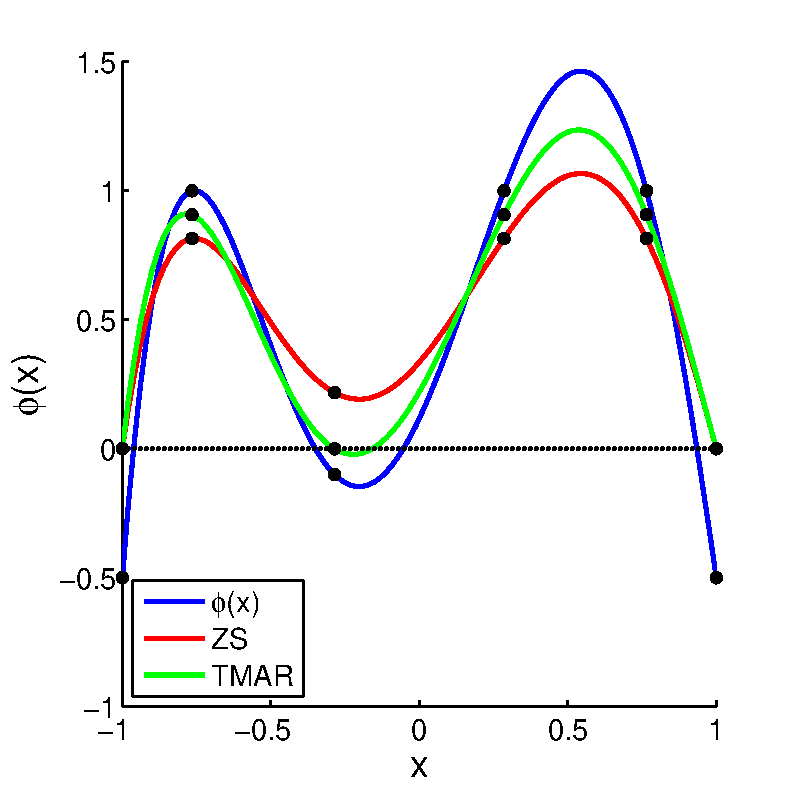
\includegraphics[width=0.5 \textwidth]{figs/1d/zsTMAR_compareEx.pdf}
\caption{Fifth degree polynomial $\phi(x)$ with three negative GLL values (blue). Linear rescaling modification to $\phi(x)$ (red). TMAR modification to $\phi(x)$ (green). GLL points shown with black dots. } \label{fig:polyModCompare}
\end{figure}

%\begin{figure}[t]
%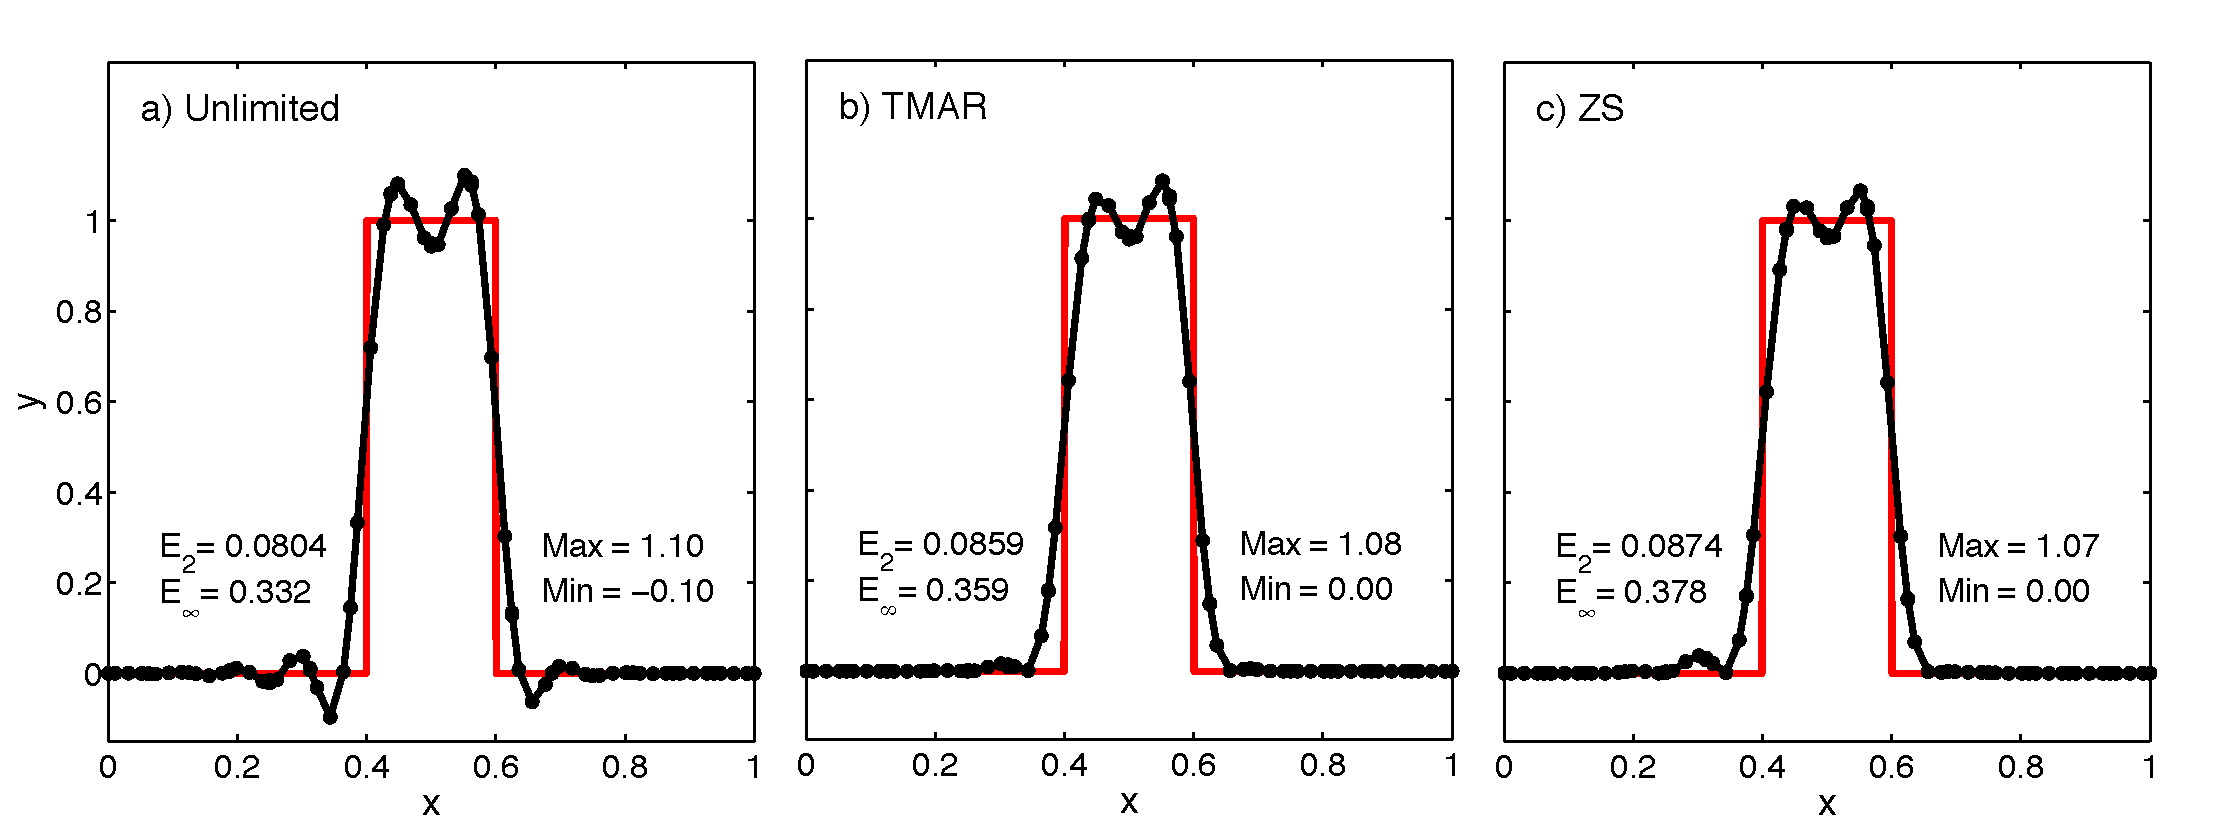
\includegraphics[width=\textwidth]{figs/1d/sqwaveCmpre_N4E16_nodal.pdf}
%\caption{Constant speed advection of a square profile five times through a periodic domain using 16 elements and 4th degree polynomials: {\bf a)} Unlimited, {\bf b)} truncated and mass-aware, and {\bf c)} Zhang and Shu solutions.} \label{fig:sqwave}
%\end{figure}

\begin{figure}[t]
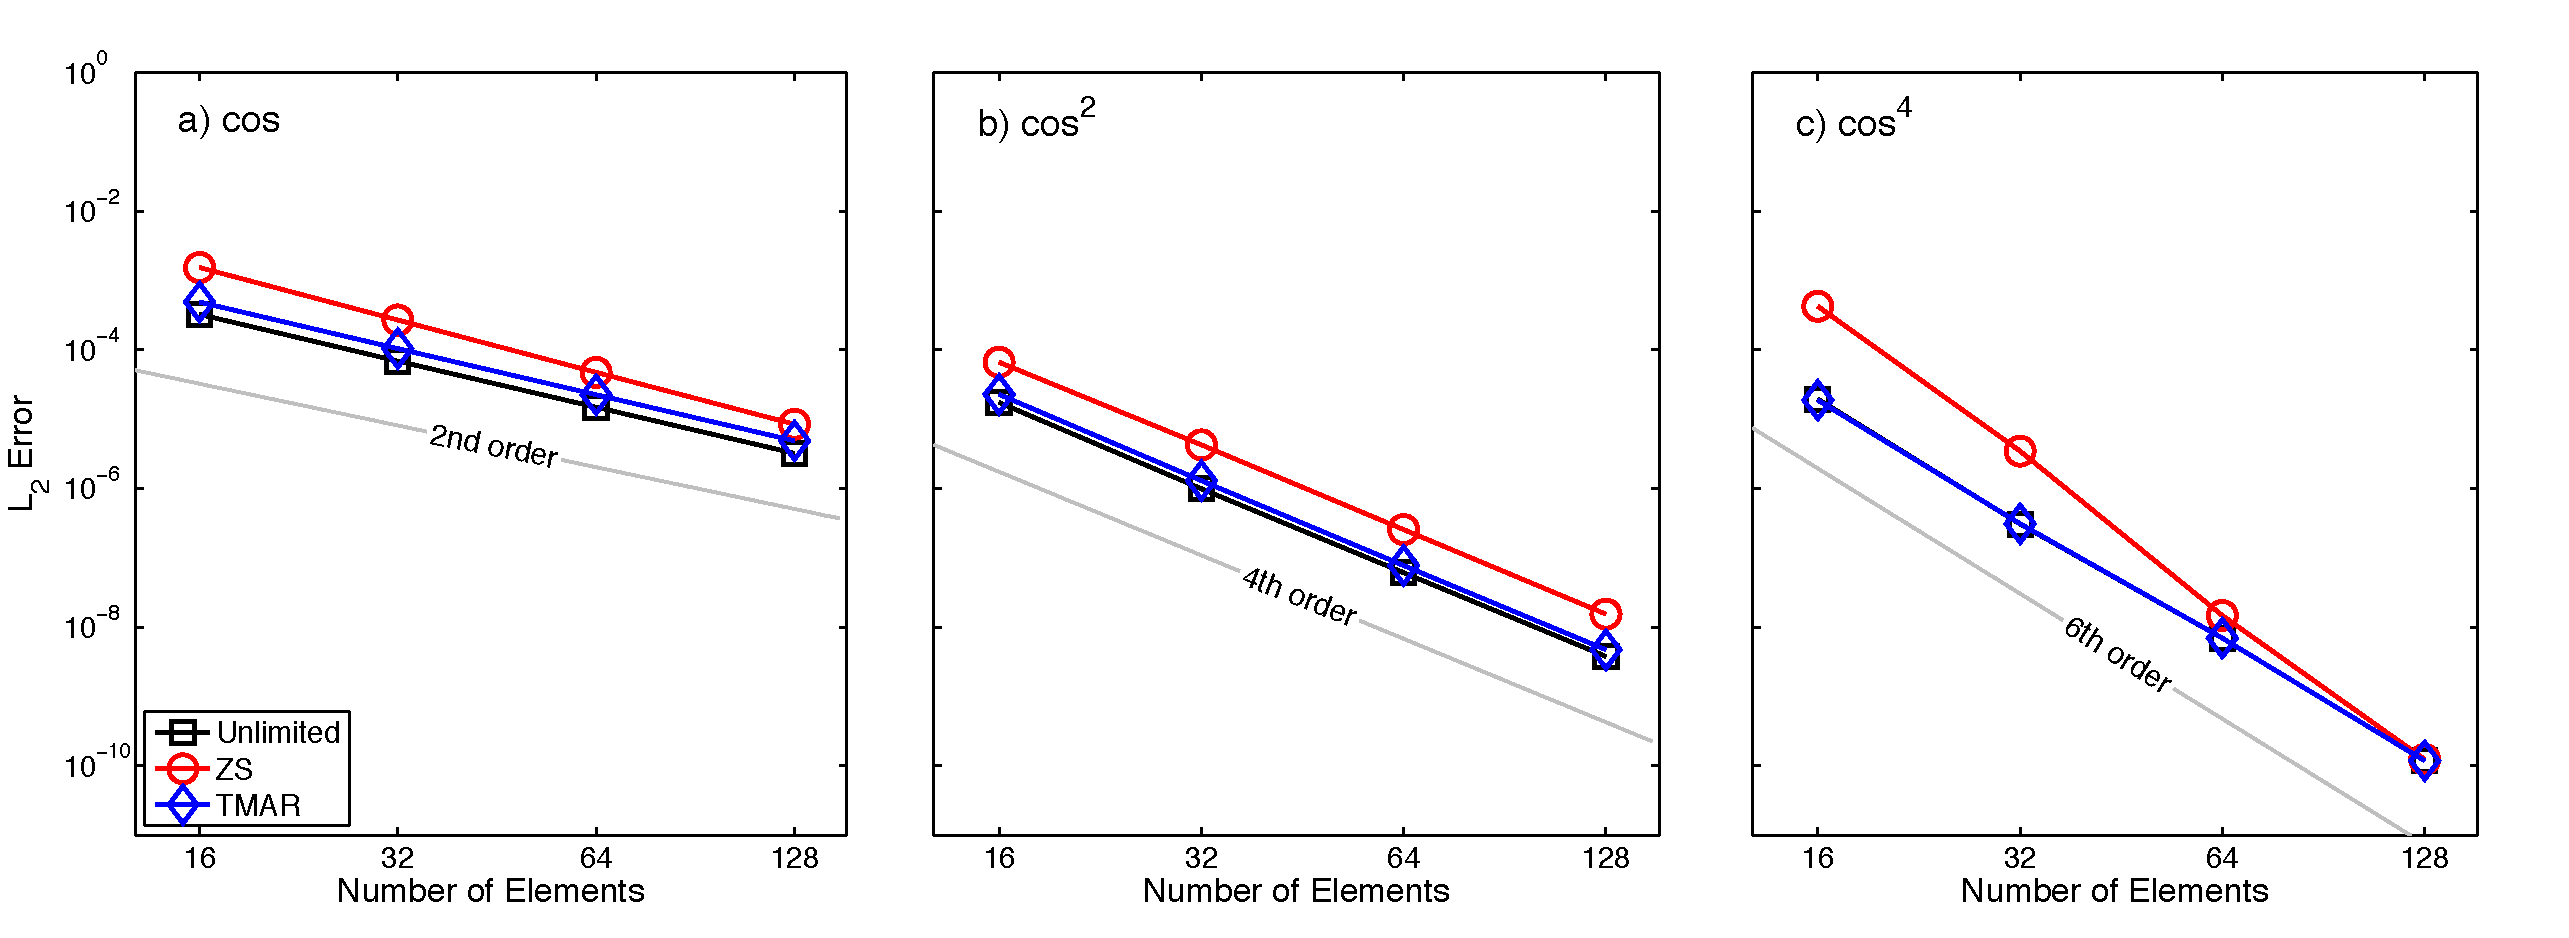
\includegraphics[width= \textwidth]{figs/1d/cosbell_hConvg_nodal.pdf}
\caption{Convergence results under $h$--refinement: log--log plot of the $L_2$ error as a function of the number of elements for {\bf a)} $C^1$, {\bf b)} $C^3$ and, {\bf c)} $C^7$ cosine bell tests with initial conditions  conditions defined in \eqref{eq:cosbell}. Each test uses $N=5$ and a time step $\dt = 0.5 \dx^{2}$. } \label{fig:cosConv-h}
\end{figure}

\begin{figure}[t]
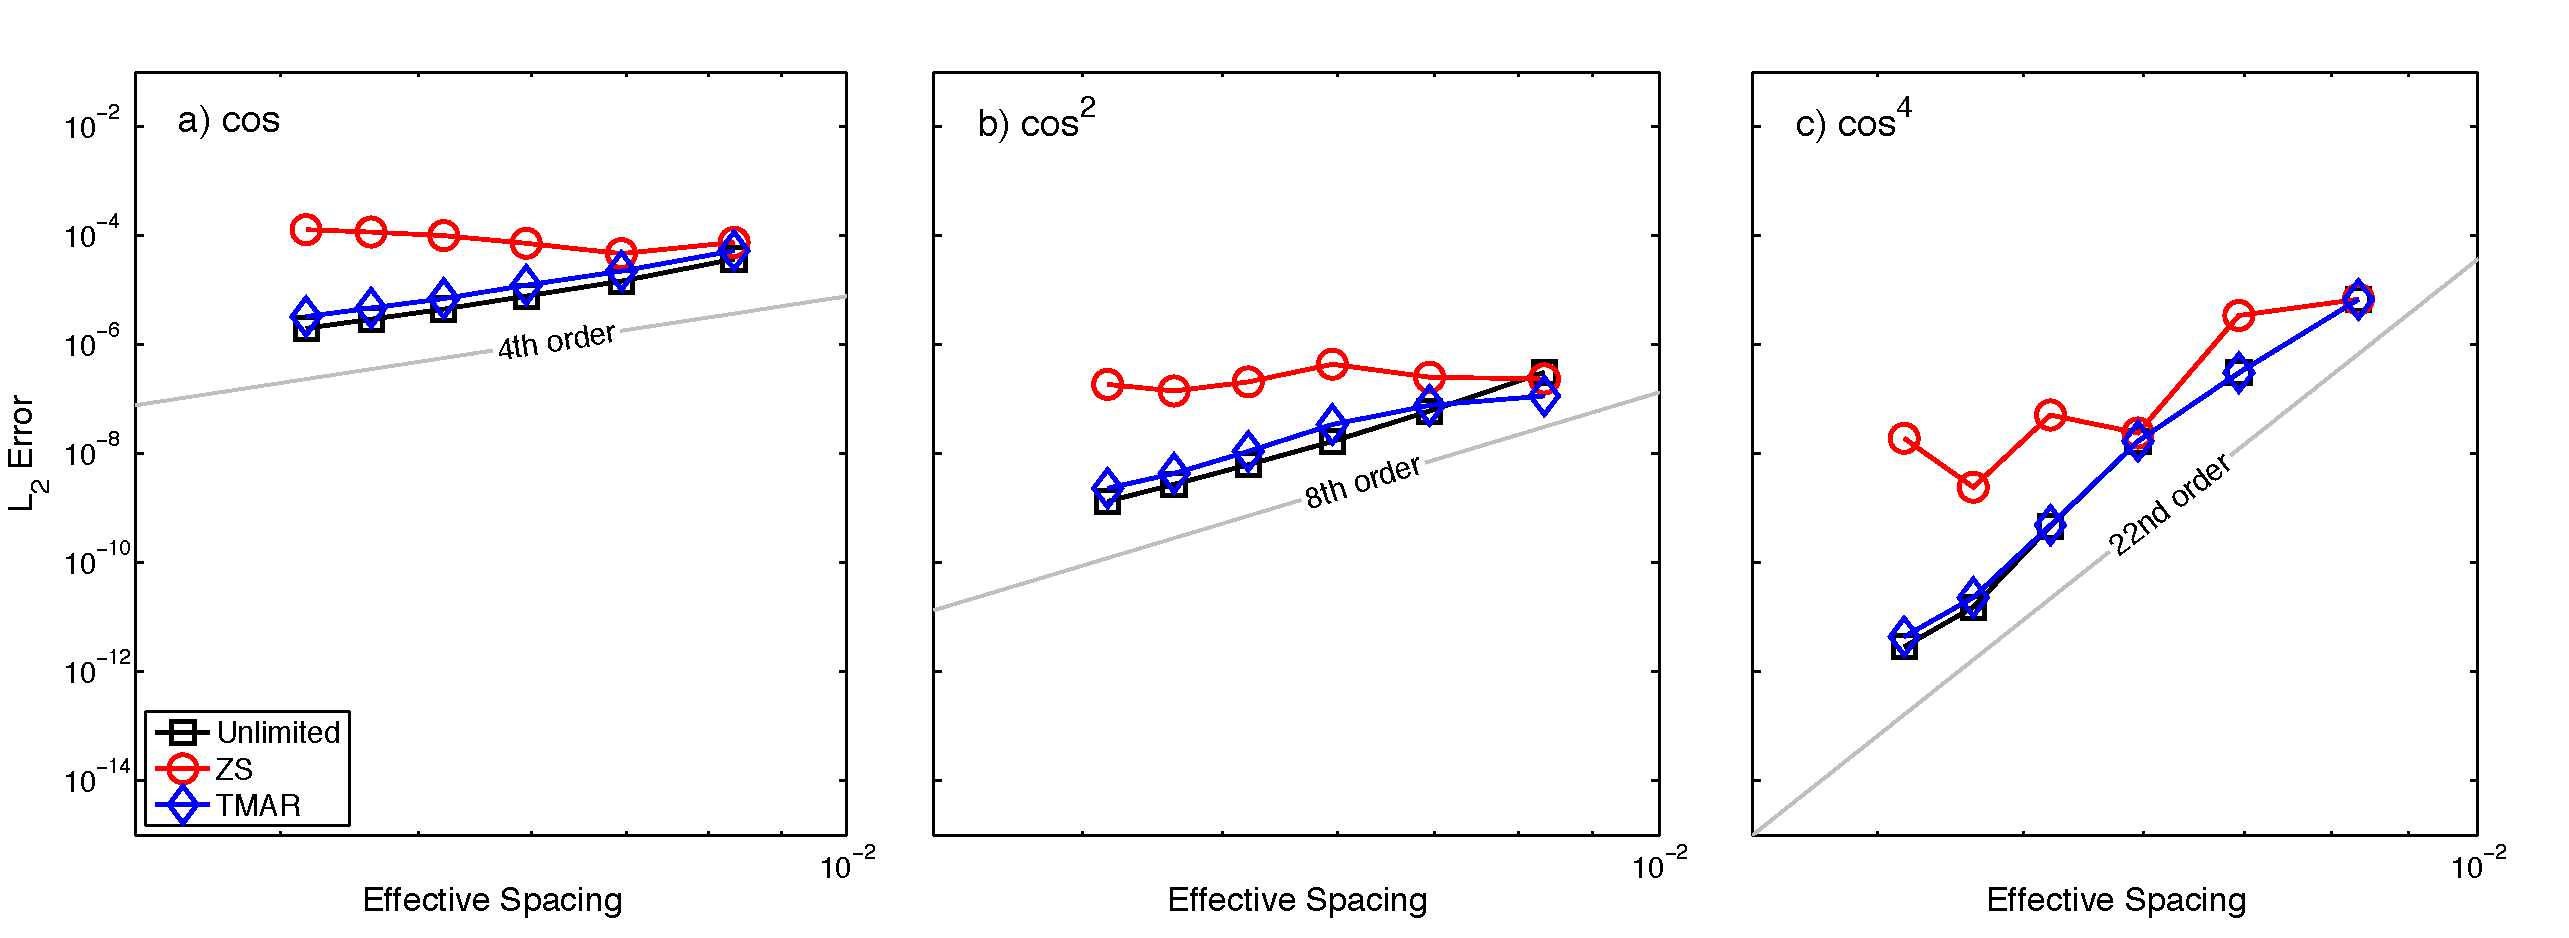
\includegraphics[width=\textwidth]{figs/1d/cosbellConvg_nodal.pdf}
\caption{Convergence results under $p$--refinement: log--log plot of the $L_2$ error as a function of the effective spacing $\widetilde{\dx}$ for {\bf a)} $C^1$, {\bf b)} $C^3$ and, {\bf c)} $C^7$ cosine bell tests. Each test uses a 32 element mesh and time step $\dt = 0.5 \dx^{(N+1)/3}$.} \label{fig:cosConv-p}
\end{figure}

\begin{figure}[t]
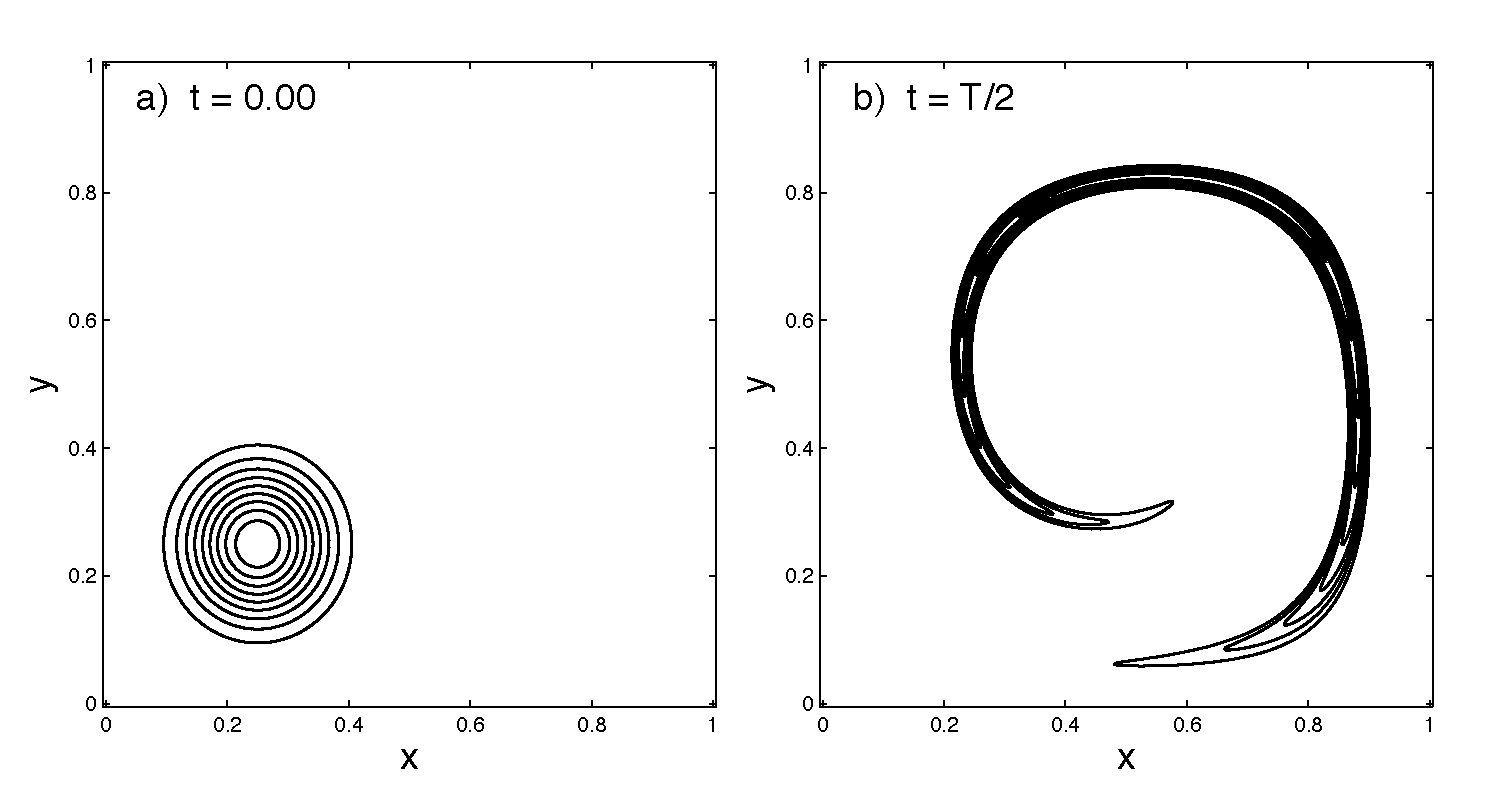
\includegraphics[width= 0.8 \textwidth]{figs/2d/defCosbellExact.pdf}
\caption{Tracer concentration field for the $C^3$ cosine bell in the reversing deformation flow \eqref{eq:2dDefVel} at times \textbf{a)} 0 and $T$, and  \textbf{b)} $T/2$. Contours at intervals of 0.1.}
\label{fig:cosbellExact}
\end{figure}

\begin{figure}[t]
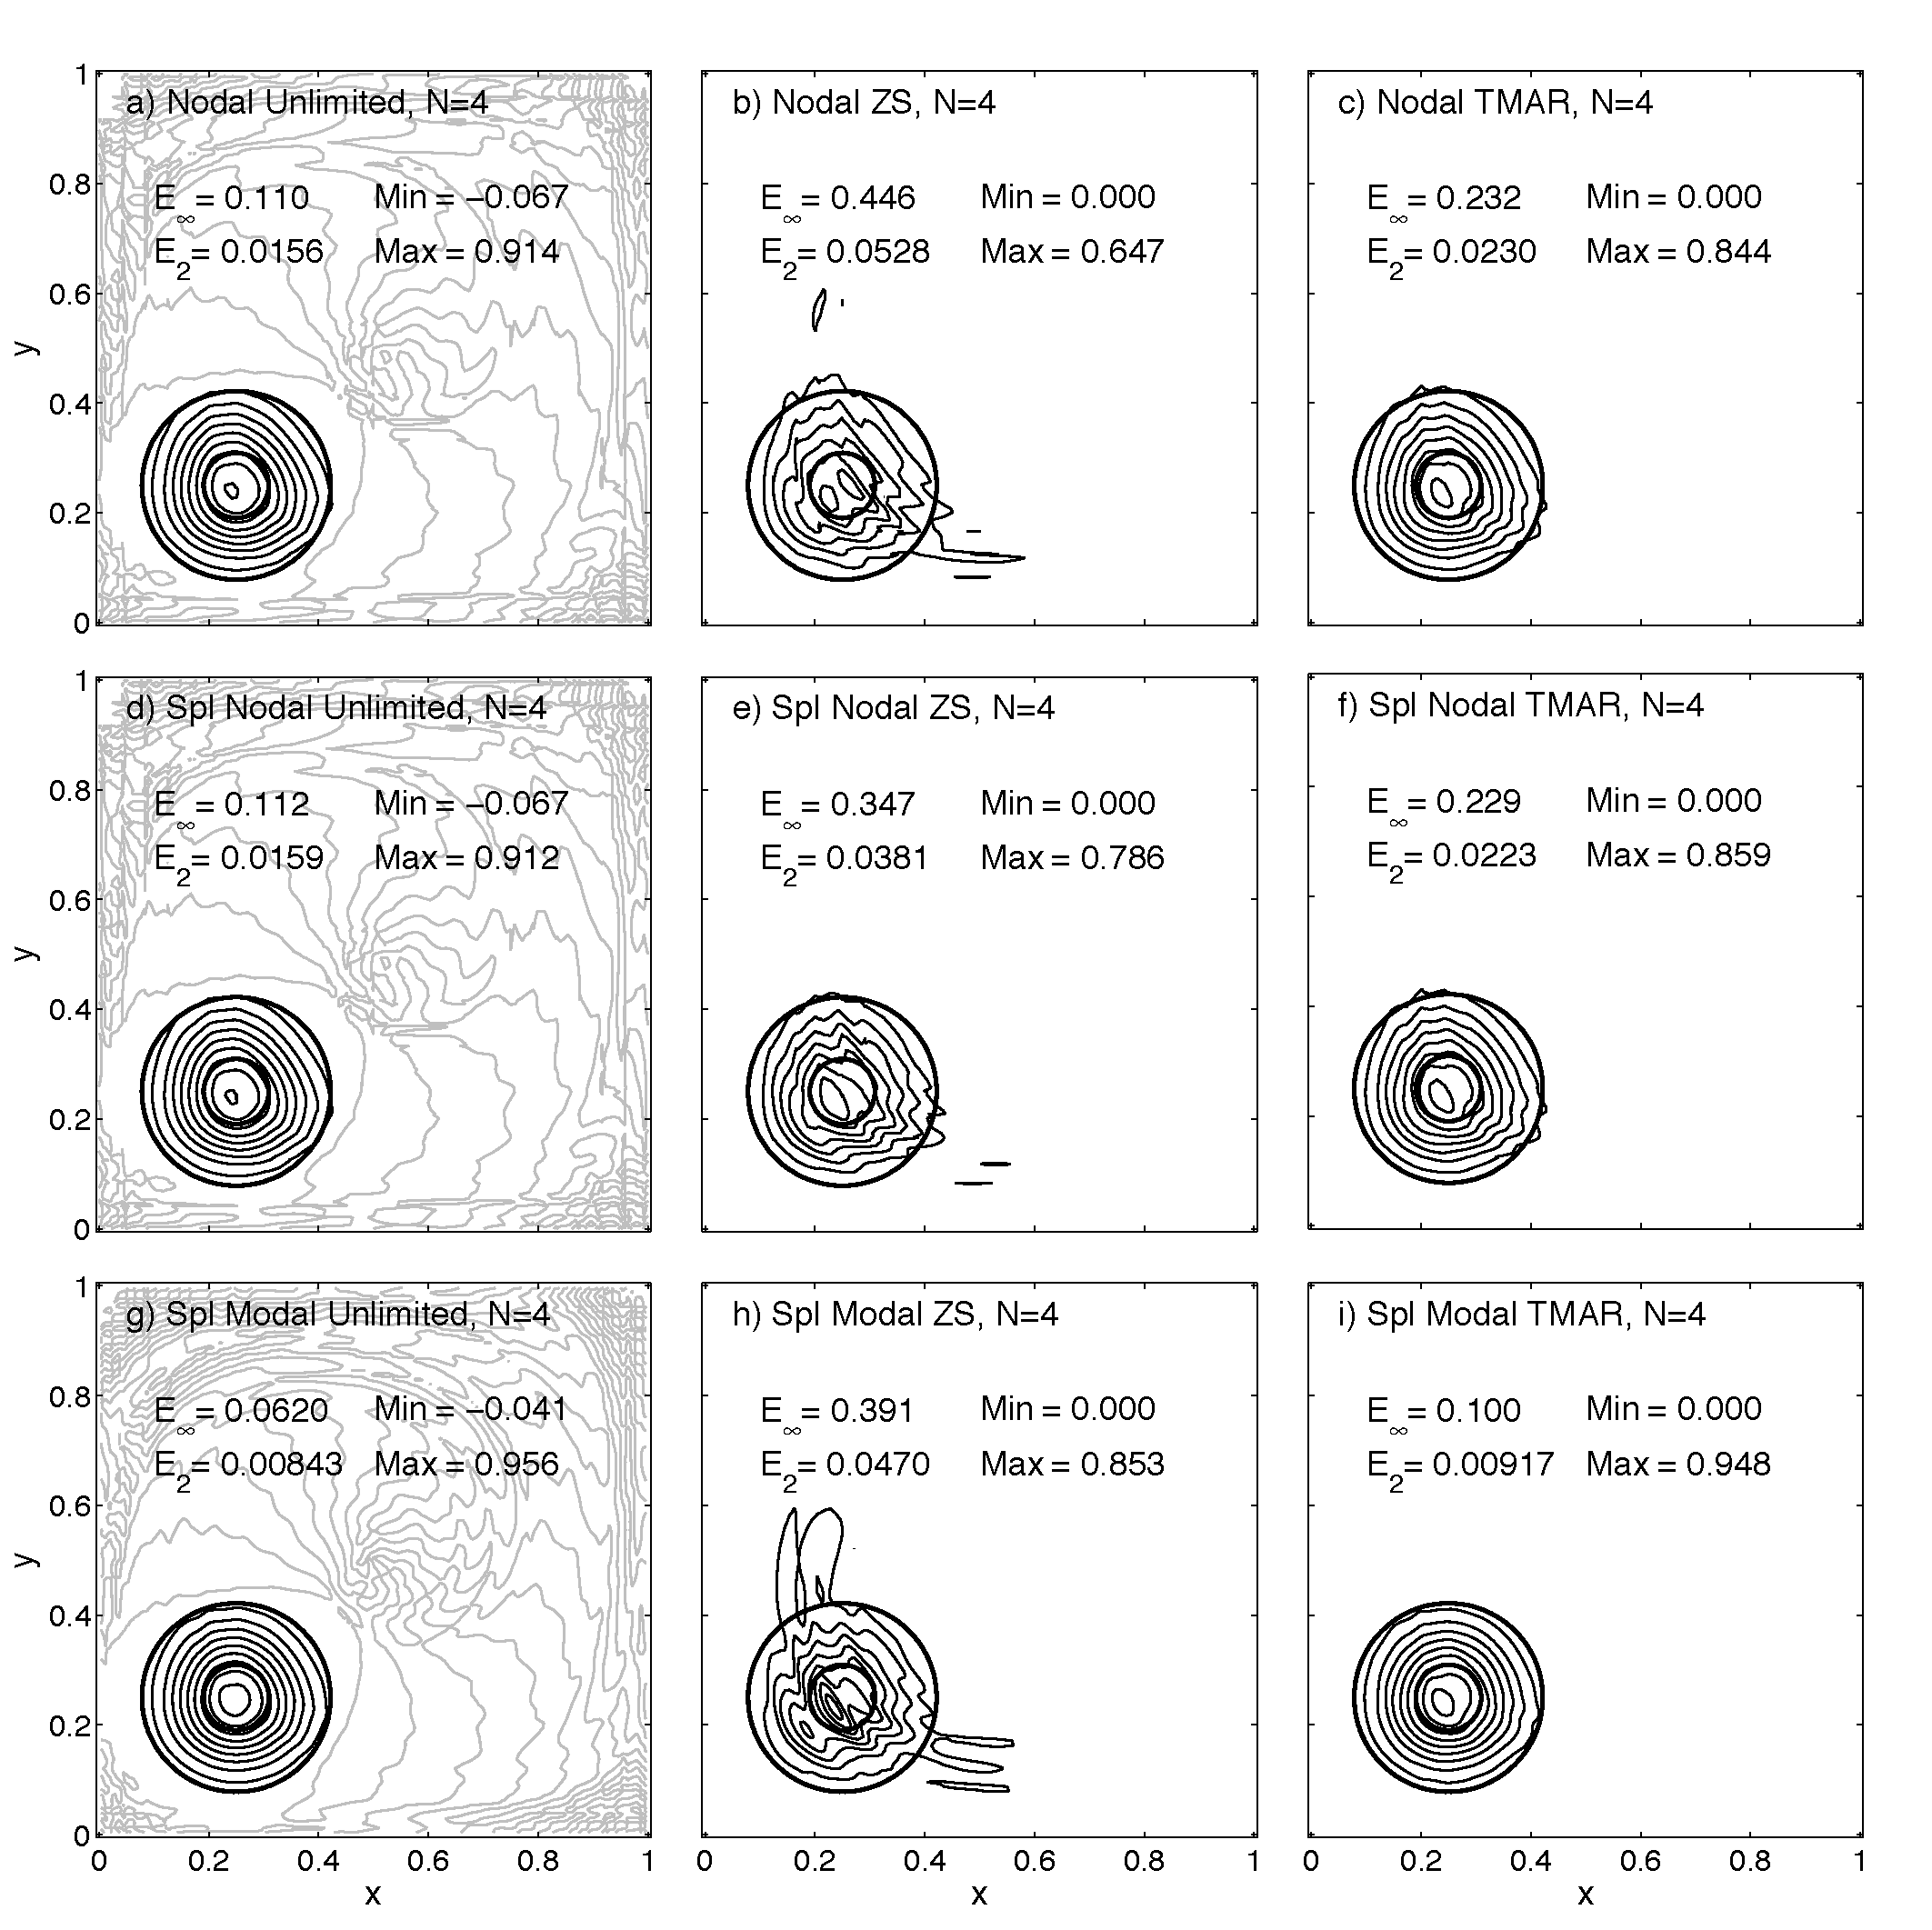
\includegraphics[width=\textwidth]{figs/2d/_defCosbell_9pan_24e.pdf}
\caption{Comparison of tracer concentration fields at $t=T$. Each panel uses the same $24\times24$ element grid. The limiting scheme and degree at which the polynomial expansions are truncated are given in each panel. Contours are every 0.1 and negative contours are highlighted in light gray. Exact solution contours at 0.05 and 0.75 shown in heavy solid lines}\label{fig:2dCosbell24}
\end{figure}

\begin{figure}[t]
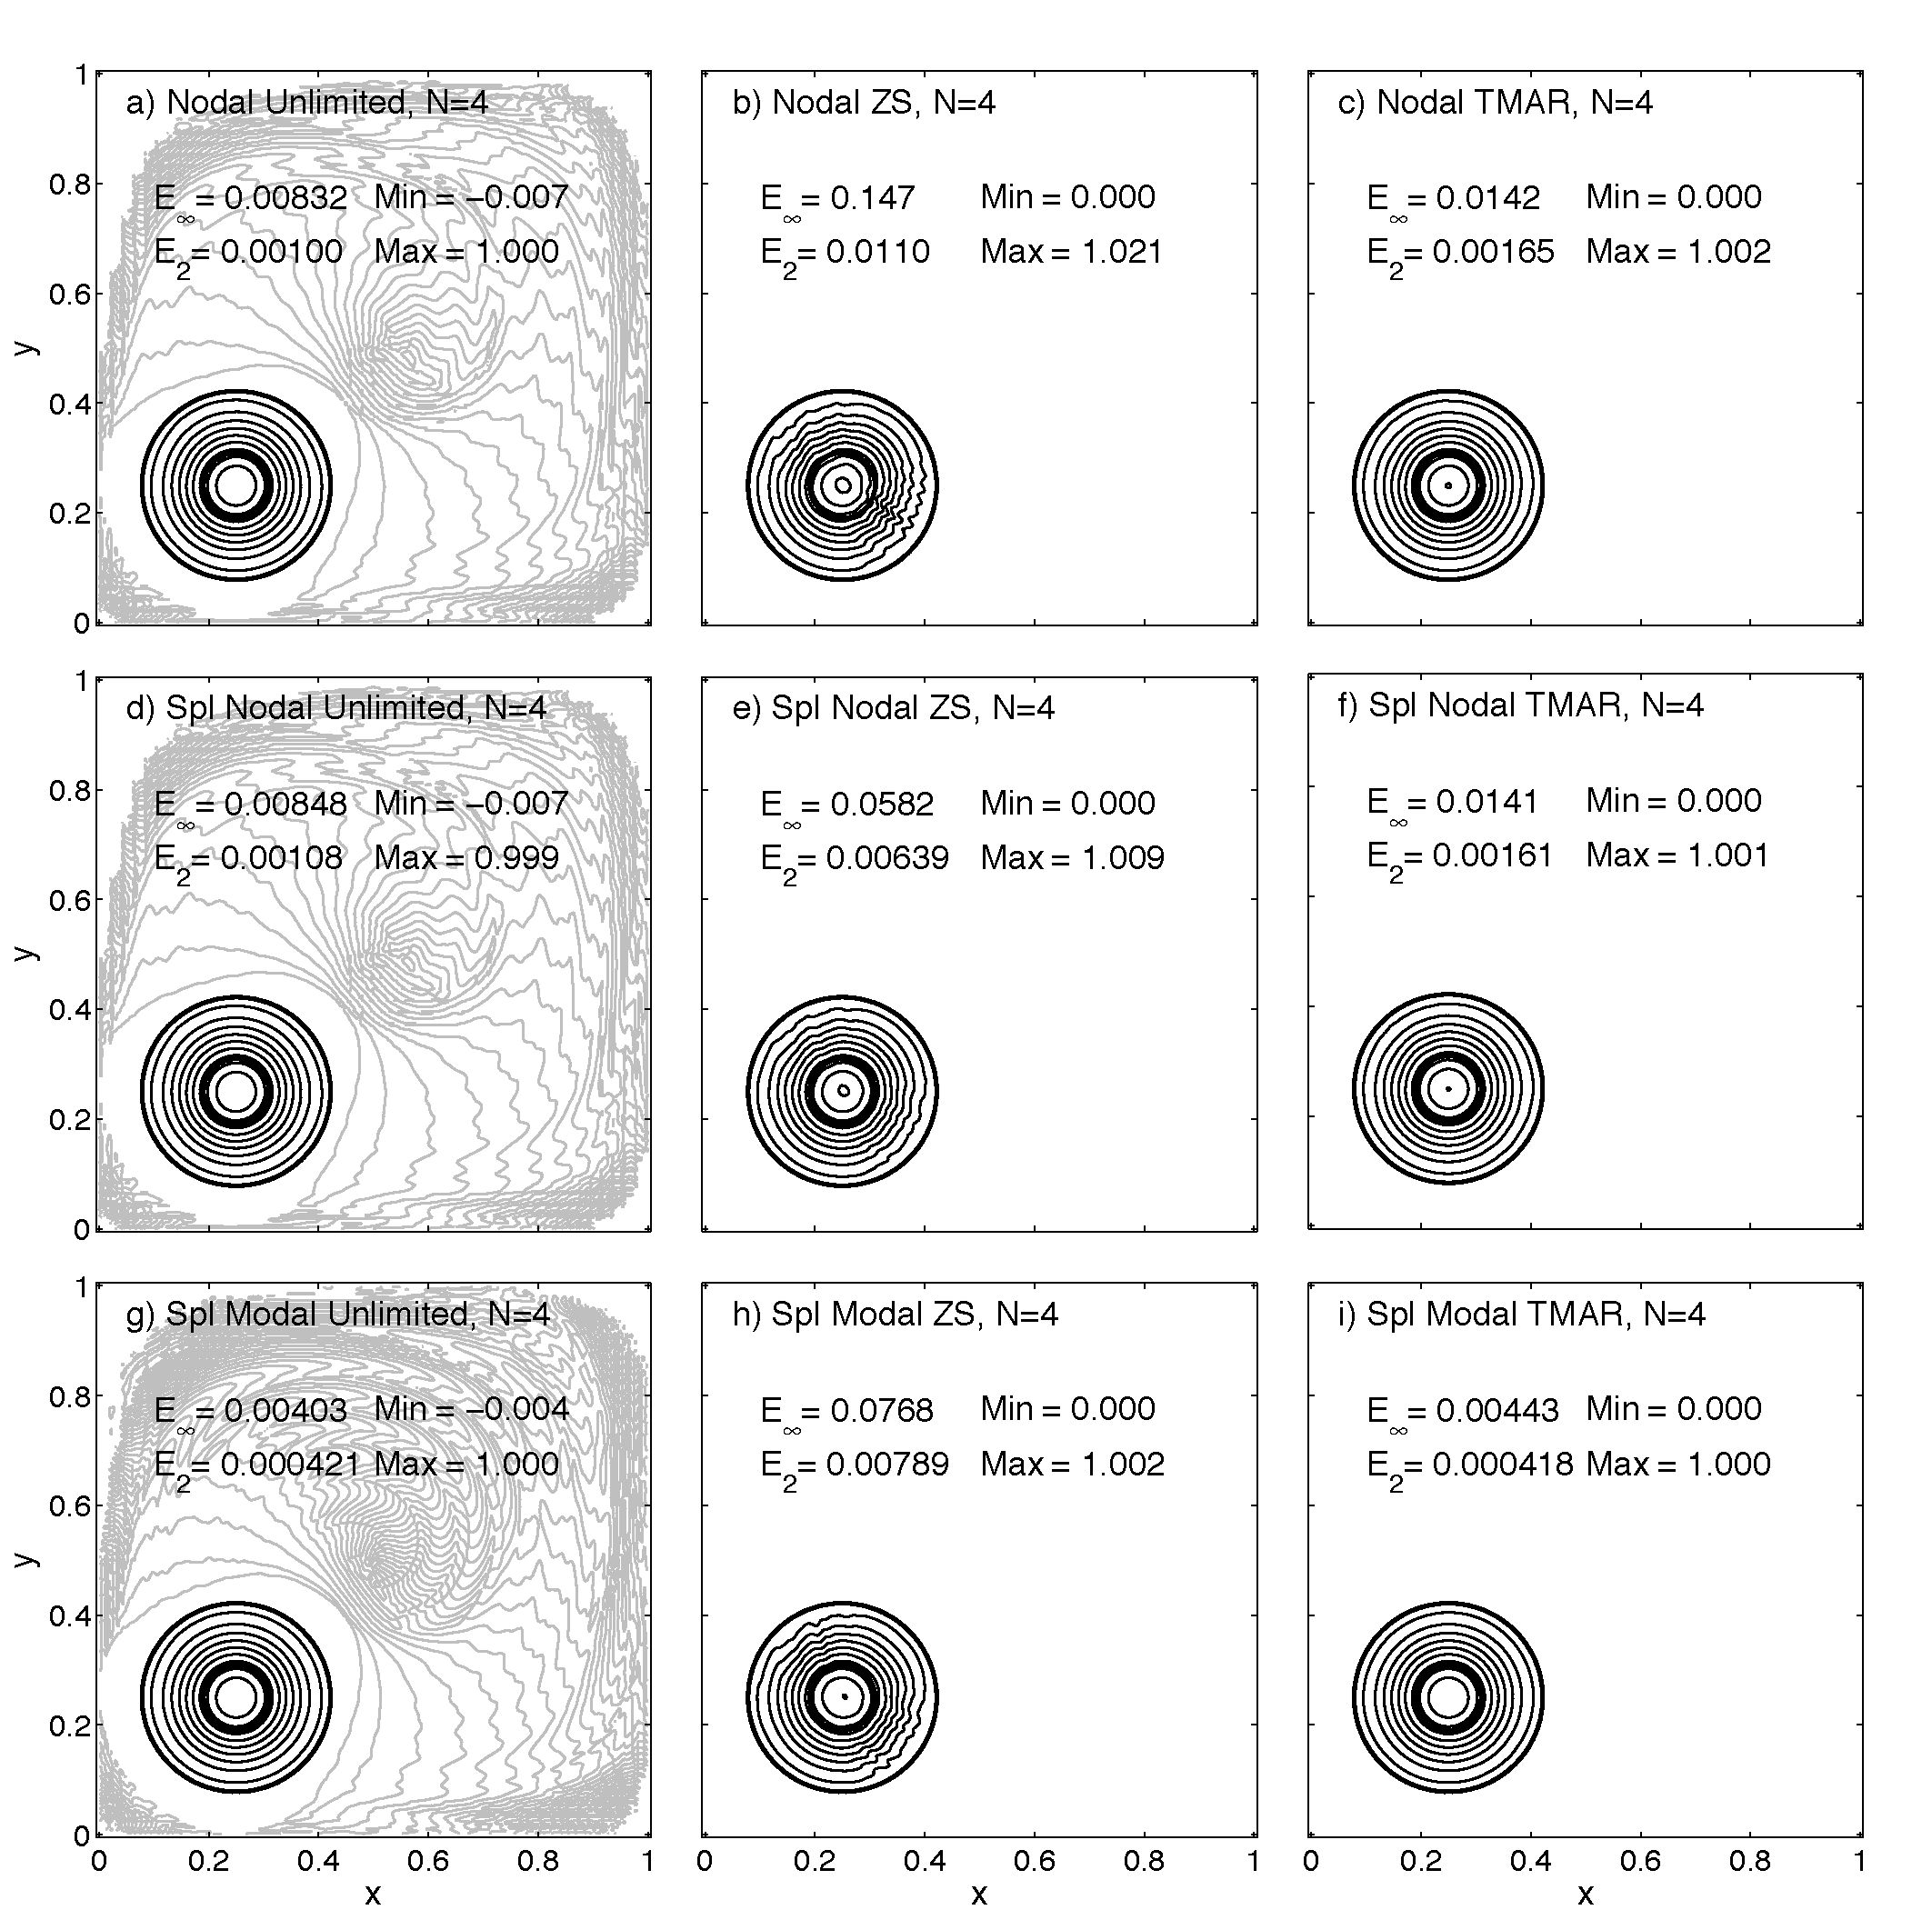
\includegraphics[width=\textwidth]{figs/2d/_defCosbell_9pan_48e.pdf}
\caption{Same as Figure~\ref{fig:2dCosbell24} but using a grid of $48\times48$ elements.}\label{fig:2dCosbell48}
\end{figure}

\begin{figure}[t]
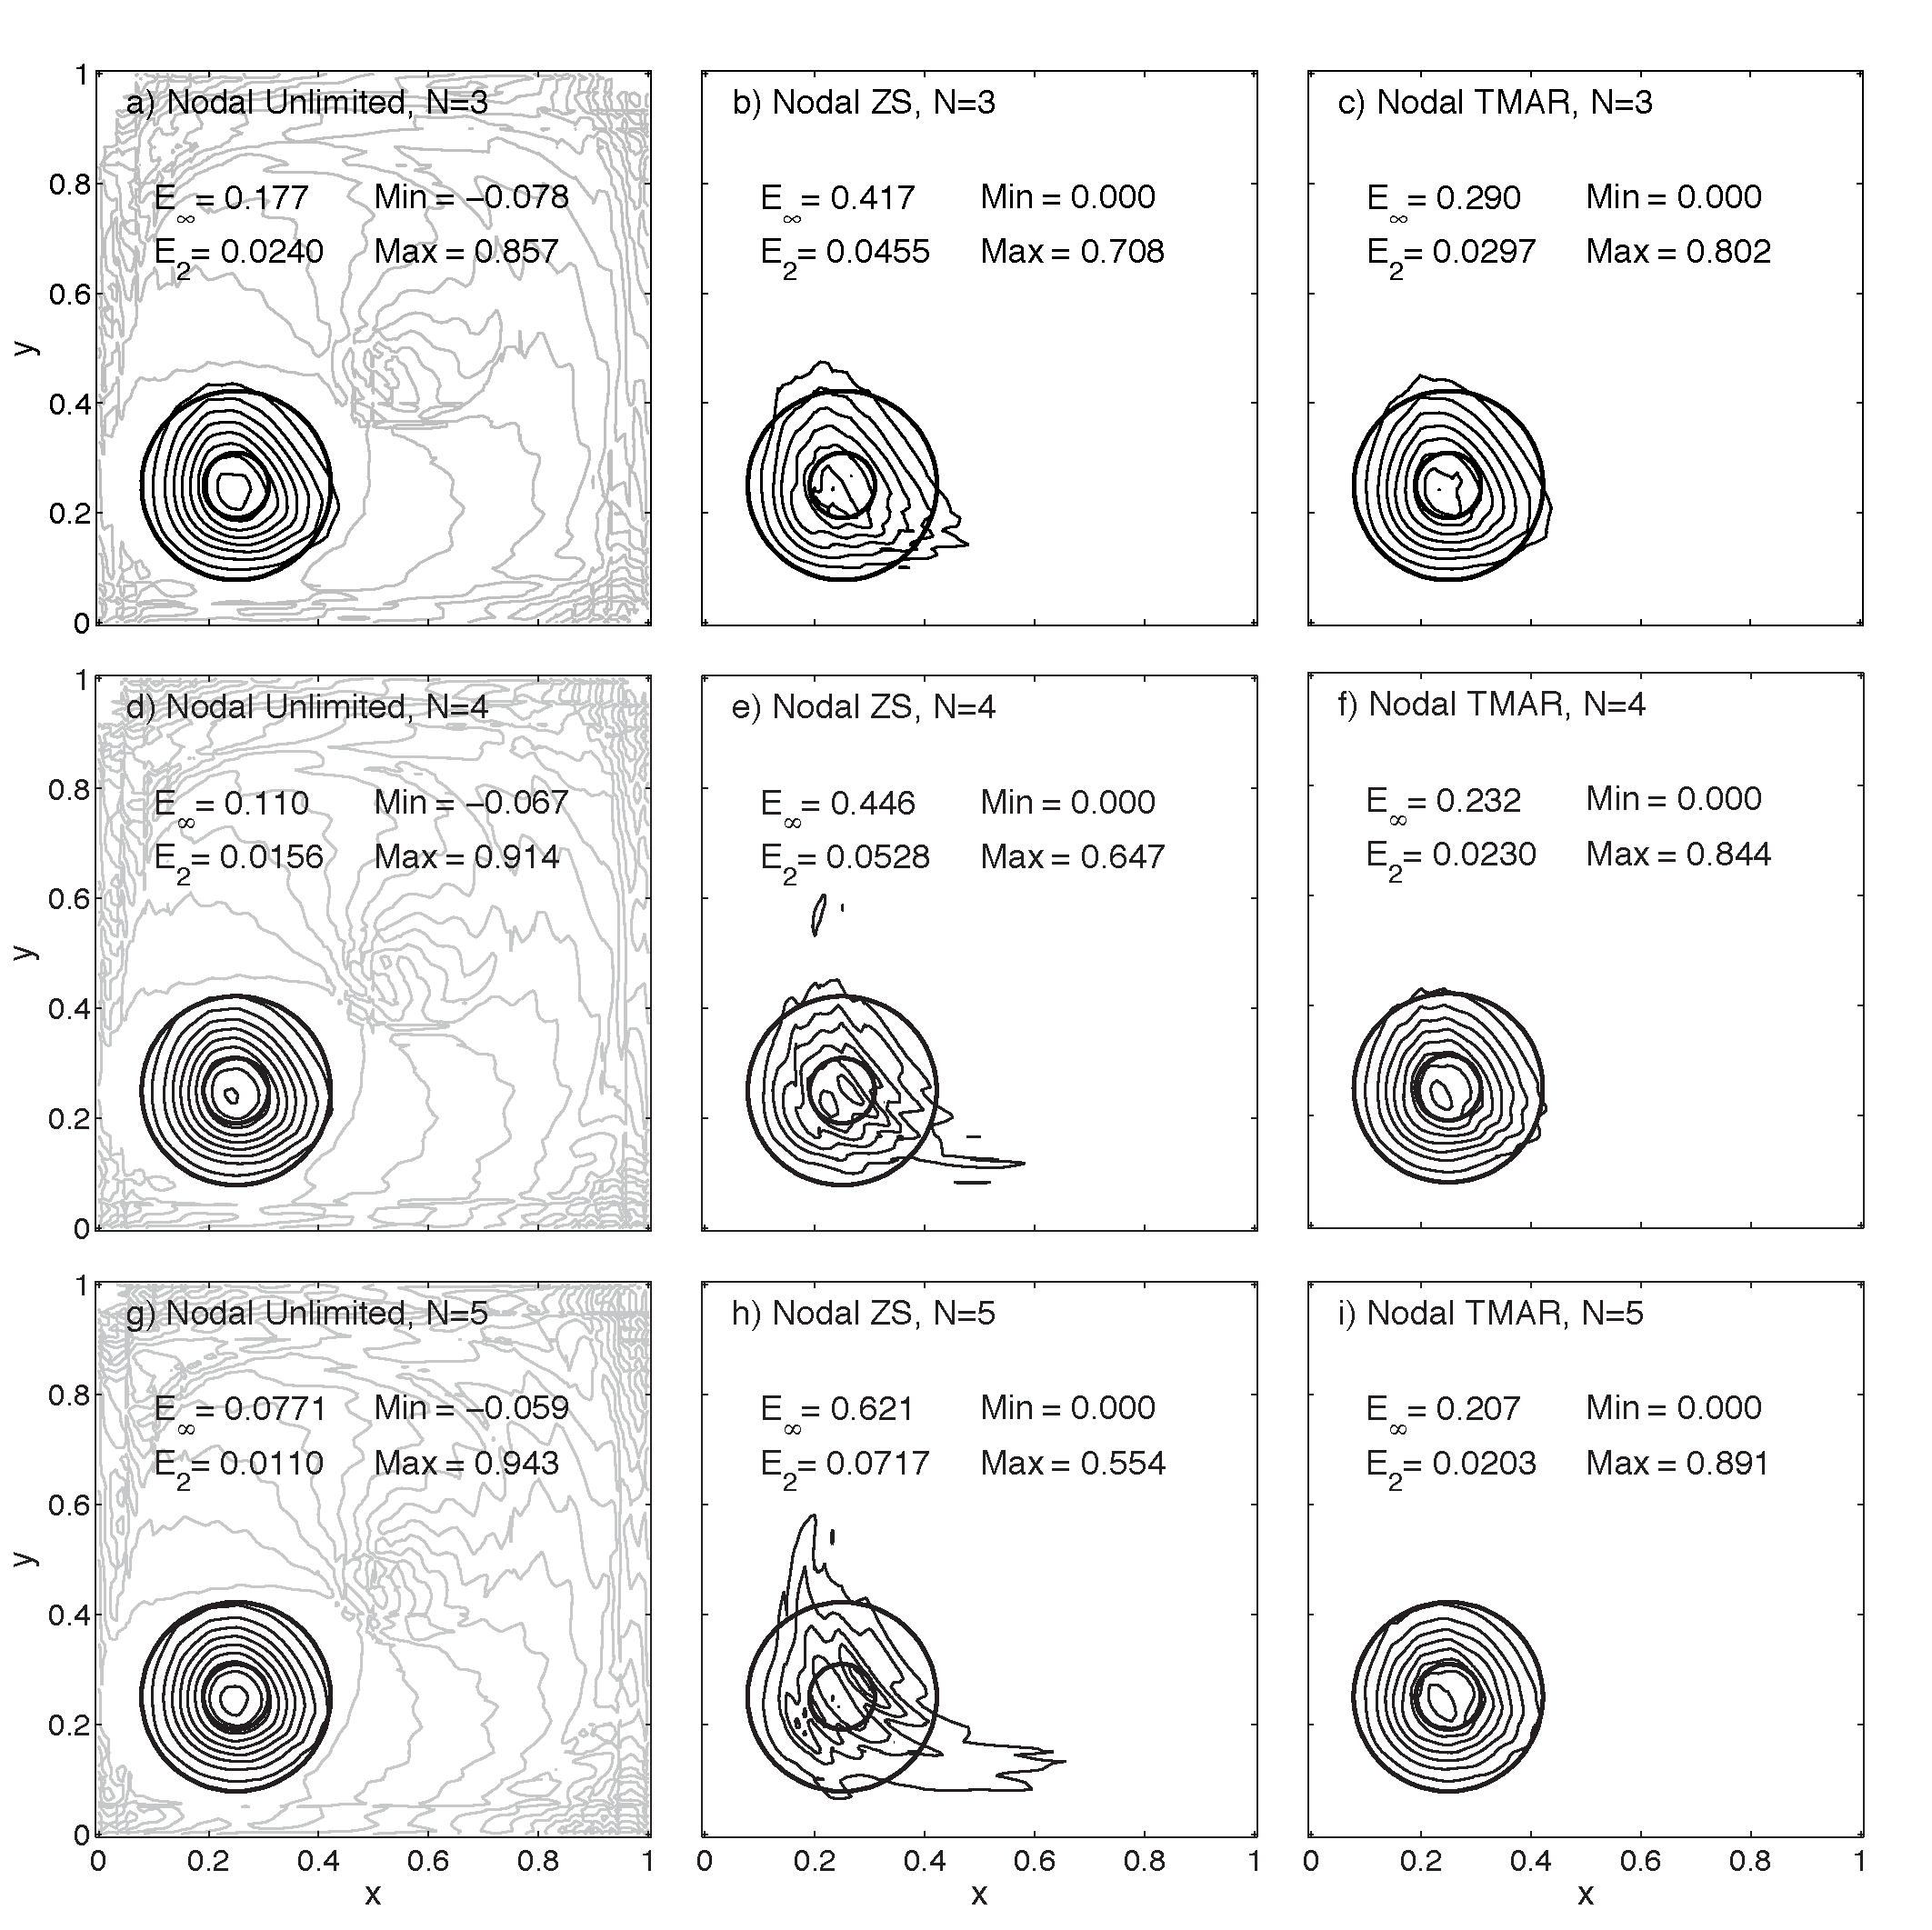
\includegraphics[width=\textwidth]{figs/2d/_defCosbell_9pan_pref.pdf}
\caption{Impact of polynomial refinement on tracer concentration fields at $t=T$. Each panel uses the same 120 total DOF along each coordinate. Limiting schemes and degree of polynomial truncation are listed in each panel. Contours are every 0.1 and negative contours are highlighted in light gray. Exact solution contours at 0.05 and 0.75 shown in heavy solid lines}\label{fig:2dCosbellPref}
\end{figure}

\begin{figure}[t]
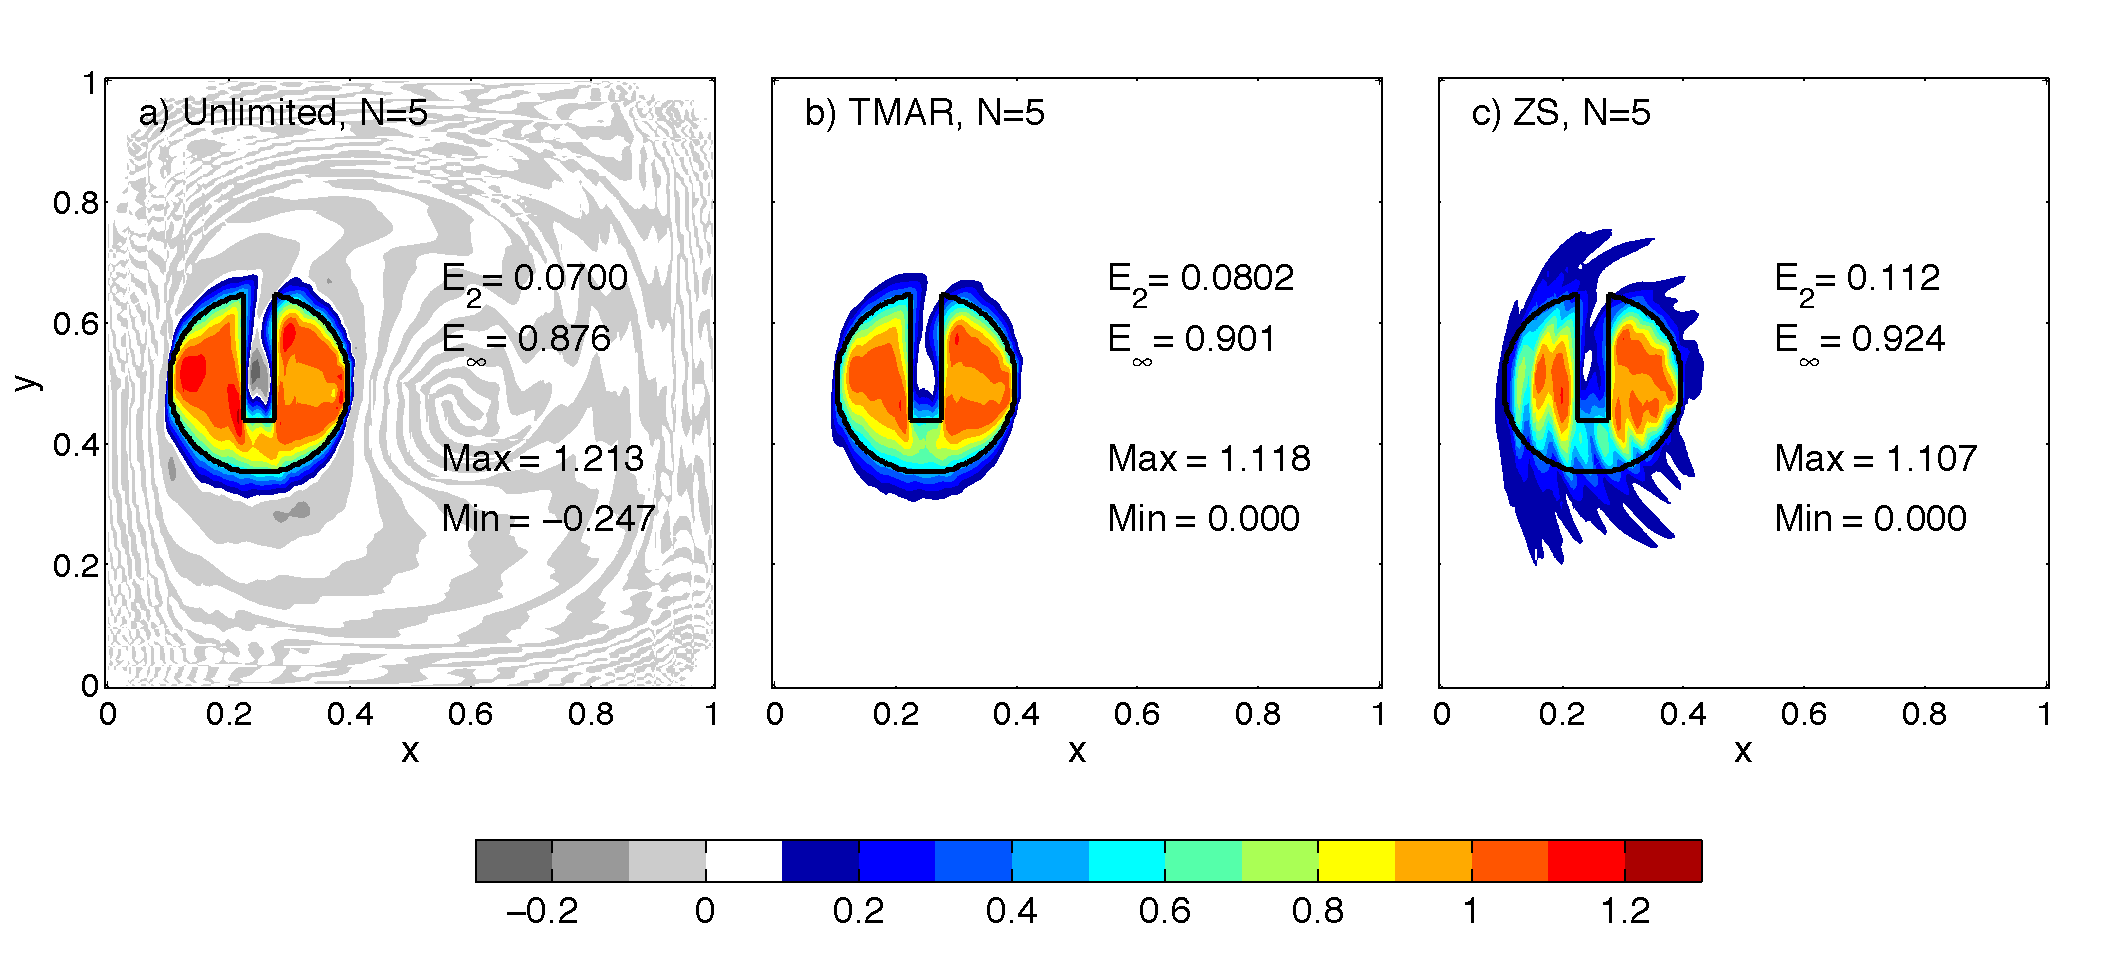
\includegraphics[width=\textwidth]{figs/2d/defCyl_3panel.pdf}
\caption{Tracer concentration field for a slotted cylinder at $t=T$. Contours are every 0.1 and negative regions are highlighted in light gray. Exact solution is outlined by the heavy solid line.}\label{fig:2dCyl}
\end{figure}

\begin{figure}[t]
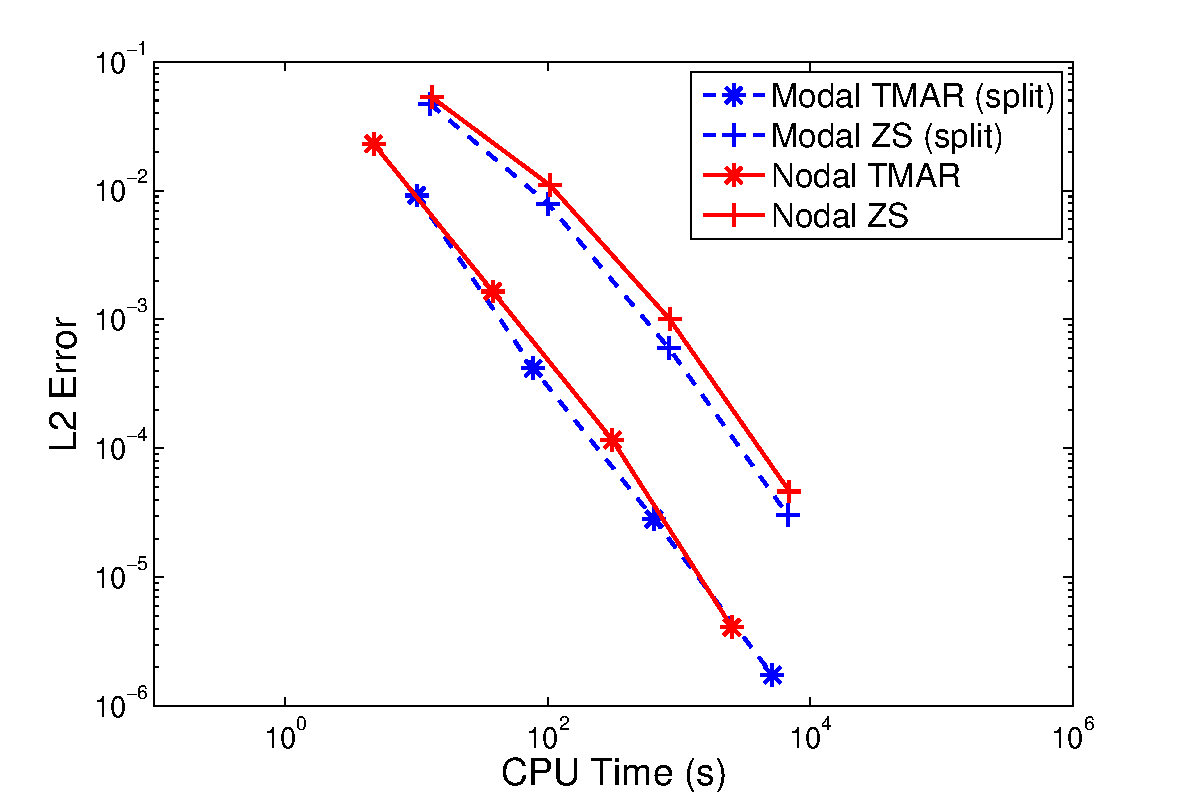
\includegraphics[width=0.7\textwidth]{figs/2d/cosbellDef_L2Cpu.pdf}
\caption{$L_2$ norm of error as a function of computational time spent to integrate the $C^3$ cosine bell deformation with $N=4$. Data points indicate numerical simulations using 24, 48, 96 and 192 elements along each coordinate. }
\label{fig:L2cpu}
\end{figure}

\end{document}